\documentclass[11pt]{article}
\usepackage[margin=1.0in]{geometry}
\usepackage[utf8]{inputenc}
\usepackage{graphicx}
\usepackage{amsmath}
\numberwithin{equation}{section}
\renewcommand{\baselinestretch}{1.5}
\usepackage{hyperref}
\usepackage[sorting=none]{biblatex}
\addbibresource{Diss.bib}

\title{Influence of the Coulomb Potential on Quantum Effects in Nonsequential Double Ionization}
\author{Gergely Eory}
\date{March 2020}

\begin{document}

\begin{titlepage}
   \begin{center}
        \vspace*{1cm}
        
        \huge
        \textbf{Influence of the Coulomb Potential on Quantum Effects in Nonsequential Double Ionization}

        \large    
        \vspace{1.5cm}
        by\\
        \textbf{Gergely Eory}\\
        \vspace{0.5cm}
        Supervisor: Dr Carla Figueira De Morisson Faria
        \vfill
            
        A thesis presented for the degree of\\
        Master in Science\\
        Theoretical Physics
            
        \vspace{0.8cm}
     
        \includegraphics[width=0.4\textwidth]{Figures/university-college-london-ucl-vector-logo-xs.png}
            
        Department of Physics and Astronomy\\
        University College London\\
        April 2020
            
   \end{center}
\end{titlepage}

\begin{center}
    \vspace*{2cm}
    \huge
    Declaration of Authorship
    \vspace{3cm}
\end{center}
\normalsize
I, Gergely Eory, declare that this thesis titled 'Influence of the Coulomb Potential on Quantum Effects in Nonsequential Double Ionization', and the work presented in it is my own. Where information has been derived from other sources, I confirm that this has been indicated in the thesis. I confirm that:
\begin{itemize}
    \item This work was done wholly or mainly while studying for a Masters degree at this University.
    \item Where any part of this thesis has previously been submitted for a degree or any other qualification at this University or any other institution, this has been clearly stated.
    \item Where I have consulted the published work of others, this is always clearly attributed.
    \item Where I have quoted from the work of others, the source is always given.
    \item Where the thesis is based on work done by myself jointly with others, I have made clear exactly what was done by others and what I have contributed myself.
\end{itemize}
\newpage
\vspace*{3cm}
\begin{abstract}
Presented in this report are my findings of my MSci research project. The Strong Field Approximation (SFA) is employed to study interference effects in Above Threshold Ionisation (ATI). Nonsequential Double Ionisation (NSDI) is an ATI phenomenon, where electron-electron correlation plays an important role in determining the dynamics of the process. Shortcomings of the application of the SFA for the treatment of the SFA is pointed out in its disregard of the effect of the Coulomb potential. Moving on, an improved model based on the SFA, the Coulomb Quantum-orbit Strong Field Approximation (CQSFA) is introduced. Analytic differences and improvements upon the SFA are investigated and discussed. Finally, a so-called Frankenstein model is explored, which seeks to include the improvements of the CQSFA model in the calculation of electron momentum distributions in NSDI. Analytic conditions on this new model's applicability are investigated, and results are presented for simple setups, involving a well-behaved subset of possible solutions. Finally, ideas for future research, and modifications for extending the applicability of the new model are discussed.
\end{abstract}
\newpage

\tableofcontents
\newpage

\section{Introduction}

Above Threshold Ionisation(ATI) is a strong-field phenomenon where an atom absorbs more photons than necessary for ionisation. This occurs in strong laser fields, where the intensity reaches $I \sim 10^{13} W/cm^2$ and higher. At such intensities, the atomic Coulomb binding potential and the laser field effects become comparable in magnitude, leading to discrepancies and the eventual breakdown of perturbation theory used in calculations. At even higher intensities, around $I \sim 10^{18} W/cm^2$, a relativistic treatment of the interaction is necessary, where the ponderomotive energy of the electron becomes comparable to the rest mass of the electron. In this project we focus on the non-relativistic regime. First, consider the ponderomotive energy and the Keldysh parameter for classification.
\par
The ponderomotive energy, $U_p$, is the cycle-averaged quiver energy of a free electron in a laser field. In a linearly polarised monochromatic laser field with angular frequency $\omega$, given by $\mathbf{E}(t) = \mathbf{E_0} sin(\omega t)$ a charged particle experiences an acceleration 
\begin{equation}
    \mathbf{a}(t) = \frac{\mathrm{d}^2 \mathbf{x}}{\mathrm{d} t^2} = \frac{q\mathbf{E}(t)}{m} = \frac{q\mathbf{E_0}}{m} sin(\omega t)
\end{equation}
\begin{equation}
    \mathbf{v}(t) = \frac{\mathrm{d} \mathbf{x}}{\mathrm{d} t} = -\frac{q\mathbf{E_0}}{m\omega} cos(\omega t)
\end{equation}
\begin{equation}
    U_p = \frac{1}{2}m \left\langle \mathbf{v}^2(t) \right\rangle_T = \frac{1}{2} m \left( \frac{q\mathbf{E_0}}{m\omega}\right)^2 \frac{1}{T} \int_0^T cos^2(\omega t) dt =\frac{1}{2} \frac{q^2 E_0^2}{ m \omega^2 }\frac{1}{T}\frac{T}{2}
\end{equation}
If we consider an electron as the particle with charge $-e$ and mass $m_e$, and employ atomic units where $\hbar = m_e = e = \epsilon_0 = k_B = 1$ this expression simplifies to
\begin{equation}
    U_p = \frac{E_0^2}{4\omega^2}
\end{equation}
In this work we only consider linearly polarised, monochromatic laser fields, and work using atomic units whenever possible.
\par
The discrepancies in ATI regime arise because the field causes a Stark shift in the energy of atomic bound states that is comparable to the photon energies. This effectively shifts the ionisation potential for electrons, leading to various ionisation mechanisms. These different mechanisms can be described by the Keldysh parameter\cite{popruzhenko_2014_invariant}, defined as $\gamma = \sqrt{\frac{I_p}{2U_p}}$, where $I_p$ is the ionisation potential. Depending on the value of the Keldysh parameter, we identify three different ionisation mechanisms: 
\begin{enumerate}
    \item Tunnel ionisation: $\gamma < 1$. \newline
    The ionisation potential is distorted by the field, narrowing the barrier and making the electron more likely to tunnel ionise.
    \item Over-the-barrier ionisation: $\gamma \ll 1$. \newline
    A low value of $\gamma$ corresponds to high $U_p$, i.e. low frequency or high intensity. In this case the electron can gain enough energy to overcome the highly distorted barrier without tunneling.
    \item Multiphoton ionisation: $\gamma > 1$. \newline
    A high value of $\gamma$ corresponds to low $U_p$, arising from a high frequency or low intensity field. A high frequency field can lead to the atom absorbing multiple photons, eventually overcoming the barrier after the absorption of n photons.
\end{enumerate}
The barrier is the effective potential given by $V_{eff} = -\frac{1}{\left| \mathbf{r} \right|} - \mathbf{r} \cdot \mathbf{E}(t)$. The first term is the atomic binding potential, while the second term is the potential due to the laser field. These processes are illustrated in Fig 1:
\begin{figure}[!htb]
    \centering
    \includegraphics[width = 12cm]{Figures/tunnelingFig.png}
    \caption{ Illustrations for (a) tunnel, (b) over-the-barrier, and (c) multiphoton ionization. The effective potential barrier $V_{eff}$ (purple) results from the field $\mathbf{F} = -\mathbf{r} \cdot \mathbf{E}$ (blue) deforming the Coulomb potential barrier V (red). As the field intensity increases, the barrier narrows and tunnelling becomes more likely. For sufficiently high intensities, the barrier is deformed such that tunnelling is not necessary for the electron to escape. Conversely, for sufficiently low intensities, the field becomes negligible and $V_{eff} \approx V$ . Each photon absorption results in a "kick" that pushes the electron towards the outside of the barrier. Image taken from the MSc thesis of Ahmed Al-Jawahiry.}
    \label{fig:barrier}
\end{figure}
\par
One of the first observed significant deviations in ATI was the plateau in the multiphoton ionisation spectrum.\cite{gpetite_1988_intensity} 
\begin{figure}[!htb]
    \centering
    \includegraphics[width=12cm]{Figures/atiSpectrum.png}
    \caption{Energy spectrum for eleven photon ionisation of Xenon using two different intensities: (a) $I = 2.2 \cdot 10^{12} W/cm^2$ and (b) $1.1 \cdot 10^{13} W/cm^2$. Image taken from (G Petite et al.)\cite{gpetite_1988_intensity}}
    \label{fig:ATISpec}
\end{figure}
Figure \ref{fig:ATISpec} shows in panel (a) that in the lower intensity regime, as expected from second order perturbation theory, which predicts an exponentially decaying envelope to the height of the peaks as the number of absorbed photons increases. In contrast, panel (b) shows a higher intensity regime where perturbation theory breaks down, and the exponential envelope is not observed at all. Here each peak corresponds to a photon absorbed in excess of what is necessary to overcome the binding potential.
The position of the peaks is given by 
\begin{equation}
    E_s = (m+s)\hbar\omega - I_p
\end{equation}
where $m$ photons are required to overcome the barrier, and $s$ is the number of photons absorbed in excess. The lower energy end of the spectrum is suppressed as the high intensity field distorts the ionisation barrier. This and similar results made it apparent that a physical theory other than perturbation theory was necessary to describe the high intensity regime.

\section{Mathematical Framework}
In this section, I will introduce some of the mathematical tools and methods used in calculations in later chapters.
\subsection{Saddle Point Approximation}\label{ch:SPA}
The Saddle Point Approximation or Method of Steepest Descent is an approximation method used to calculate integrals\cite{maxwell_2019_strongfield}. It is a very useful tool for the calculation of quantum mechanical integrals formulated in terms of an action. In the context of ionisation it carries the added benefit of providing semiclassical equations of motion for the electrons, which lead to different 'quantum trajectories', discussed in the next subsection. These trajectories will be instrumental later in the calculation of ATI transition amplitudes. 
\nelwline
The approximation can be applied to integrals in the form 
\begin{equation} \label{eq:2.1}
    I(\lambda) = \int_{-\infty}^{\infty} dx F(x) e^{i\lambda S(x)}
\end{equation}
if $\lambda$ is large, and $F(x)$ is slowly varying compared to the rest of the integrand. The method works by taking the second order Taylor expansion of the function $S(x)$ about the stationary (saddle) point(s) $x_s$, i.e. $S'(x_s) = 0$, so that
\begin{equation}
    S(x) \approx S(x_s) + \frac{S''(x_s)}{2}(x-x_s)^2
\end{equation}
Inserting into Eq.S (\ref{eq:2.1}), it gives
\begin{equation}
    I(\lambda) \approx \sum_s F(x_s) e^{i\lambda S(x_s)} \int_{-\infty}^{\infty} dx  exp[i\lambda \frac{S''(x_s)}{2}(x-x_s)^2]
\end{equation}
The Gaussian integral can be carried out analytically, which leads to
\begin{equation} \label{eq:I_lambda}
    I(\lambda) \approx \sum_s \sqrt{\frac{2\pi}{i\lambda S''(x_s)}} F(x_s) e^{i\lambda S(x_s)}
\end{equation}
The term $\sqrt{\frac{2\pi}{i\lambda S''(x_s)}} F(x_s)$ is often called the prefactor, and is dealt with separately to the complex exponential part of the integral. If the action is integrated over multiple variables, one can extend the method to a multivariate Gaussian integral which takes the form
\begin{equation} \label{eq:2.5}
    I(\lambda) = \prod_{n=1}^N \left (\int_{-\infty}^{\infty} dx_n \right ) F(x_1,...,x_N) e^{i\lambda S(x_1,...,x_N)}
\end{equation}
which leads to N saddle point equations
\begin{equation}
    \frac{\partial S}{\partial x_1} = 0, ... , \frac{\partial S}{\partial x_N} = 0
\end{equation}
Expanding in a multivariate Taylor expansion and computing N Gaussian integrals leads to
\begin{equation}
    I(\lambda) \approx \left ( \frac{2\pi}{i\lambda}\right )^{\frac{N}{2}} \sum_s (det[S''(x_{1s},...,x_{Ns})])^{-1/2} F(x_{1s},...,n_{Ns}) exp [i\lambda S(x_{1s},...,x_{Ns})]
\end{equation}
where $S''(x_{1s},...,x_{Ns})$ is the Hessian matrix of the multivariate action. 
\newline
To use the Saddle Point Approximation in path integral methods, one needs to generalise Eq. (\ref{eq:2.5}) in functional form as
\begin{equation}
    I(\lambda) = \int \mathcal{D} F[x] e^{i\lambda S[x]}
\end{equation}
The saddle point equations can then be written in a functional form as $\delta S[x_s] = 0$, which using the calculus of variations leads to the Euler-Lagrange or Hamilton's equations. Performing a similar second order Taylor expansion as previously, and denoting $\delta x(t) = x(t) - x_s(t)$, the functional integral can be approximated as 
\begin{equation}
    I(\lambda) \approx \sum_s F[x_s] \left [ det \left (- \frac{\delta^2 S}{\delta x(t) \delta x(t')}\right )\right ] ^ {-1/2} e^{i \lambda S[x_s]}
\end{equation}
The functional derivative inside the determinant will reduce to a differential operator. It is difficult to compute in general, but if one is dealing with an action for a real system with meaningful definitions for position and momentum, the above equation can be written as
\begin{equation}
    I(\lambda) \approx \sum_s F[x_s] \left [ det \left (- \frac{\partial p_s(t_f)}{\partial x_s(t_i)}\right )\right ] ^ {1/2} e^{i \lambda S[x_s]}
\end{equation}
where $t_i$ and $t_f$ denote the final and initial times, respectively. In three spatial dimensions, this expression requires one to calculate the derivative of a $3 \times 3$ matrix, which is much easier to calculate. 
\subsection{Quantum Orbits}\label{ch:QO}
Solving the saddle point equations i.e. finding stationary points of the action, lead to solutions known as quantum orbits or quantum trajectories. They are governed by classical equations of motion derived from the saddle point equations, but they can account for intrinsically quantum behaviour, such as quantum tunneling and interference. The tunneling is possible as the equations are usually extended to the complex plane leading to non-classical effects. In the case of tunnel ionisation (and most other semi-classical descriptions of tunnelling), the time of ionisation is complex and propagation parallel to the imaginary axis to get to the real time axis is what results in the tunnelling of the electron. Similarly, the complex valued solutions corresponding to multiple quantum trajectories can lead to interference.
\par
It is important to note that quantum orbits provide a self consistent "physical" picture of the physics governing the ionisation processes, but the trajectories themselves are not "physical" and cannot be observed or measured. Only the final transition amplitude, which is a combination of all possible trajectories corresponds to a physical observable.

\section{Nonsequential Double Ionisation} \label{ch:NSDI}
\subsection{History}
Nonsequential Double Ionisation (NSDI) is a phenomenon that can take place when there are two active electrons simultaneously in the ionisation process. In this phenomenon, the two electrons have a strong correlation by the time ordering of their respective ionisation, which is then manifest in their final measured momentum distributions.
\par
In 1984, the NSDI was first predicted\cite{lhuillier_1983_multiply} in the multiphoton ionisation regime $(\gamma > 1)$, when the ionisation cross-section of Xe atoms was investigated in a high intensity external laser field. In this paper two processes were considered. A sequential process, where one electron ionises from the ground state of the atom, then another ionises from the ground state of the ion, without any interaction between the two electrons. The other one was a nonsequential process, where two electrons were ionised simultaneously from the ground state of the atom.
\par
The NSDI was later observed to be present not only in the multiphoton regime, but in the tunneling ionisation regime $\gamma \ll 1$ as well. Experiments have shown a structure dubbed "the knee"\cite{walker_1994_precision}, which is a multiple order of magnitude deviation from predictions based on sequential models in the double ionisation yield of Ne and He as a function of driving field intensity. This structure is illustrated in Fig \ref{fig:knee}.
\begin{figure}[!htb]
    \centering
    \includegraphics[width=10cm, height=12cm]{Figures/theKnee.png}
    \caption{Measured ionization yields as functions of the laser intensity for double ionization of helium at 780 nm. The crosses represent the experimental results and the rest theoretical calculations. For He2+ the solid and dot lines show the calculations for sequential and nonsequential (NS) double ionization, respectively.Image taken from (Walker et al.)\cite{walker_1994_precision}}
    \label{fig:knee}
\end{figure}
The presence of "the knee" in the double ionisation yield of multiple atoms and molecules lead to the conclusion that electron-electron dynamics is responsible for NSDI process. The physical mechanism behind NSDI was, however, still unknown. Multiple processes were proposed to explain nonsequential double ionisation for a low frequency, high intensity field\cite{tahirshaaran_2011_a}, such as collective tunneling where both electrons tunnel-ionise simultaneously. Another proposition was a shake-off process where one electron ionises, and due to the sudden rearrangement of the electronic structure, a second electron is promoted to an excited state, from which it immediately ionises. These processes both lead to the expectation that the electrons would be most likely to ionise at a field maximum, when the potential barrier is the most distorted. If this were the case, one would expect the momentum distributions of the electrons at the detector to be centred at 0. This would correspond to tunneling with vanishing momentum component parallel to the laser field, then propagating to the detector.
\par
Further evidence for the nonsequential process was found when the cold-target recoil ion momentum spectroscopy (COLTRIMS) technique was developed\cite{ullrich_2003_recoilion}, which enabled one to measure electron momentum distributions as functions of electron momenta parallel to the laser field polarisation\cite{a2011_electronelectron}. Such distributions were peaked at nonvanishing parallel momenta, which indicated that both electrons left preferably at the crossing of the laser field. These results contradicted the models of collective tunneling and the shake-off process. Instead, this new piece of evidence was in favour of another proposed model, called the three-step model.

\subsection{Three-Step Model}\label{ch:TSM}

A process based on rescattering was also proposed\cite{corkum_1993_plasma}, which postulates a three-step model to explain the physical mechanism behind NSDI:
\begin{itemize}
    \item Near the maximum of the external laser field, the first electron tunnel-ionises through the distorted potential well of the atom. After ionisation, the electron propagates in the continuum, governed by its initial momentum and its interaction with the field.
    \item After the field crossing, the electron is accelerated back to the parent ion, and gains additional kinetic energy from the field.
    \item Upon return to the core, the electron collides with its parent ion, which may lead to different physical processes. The electron may:
    \begin{itemize}
        \item recombine with the parent ion and emit energy in the form of high order harmonics, leading to a process called High Harmonic Generation (HHG).
        \item scatter elastically with the core before reaching the detector, leading to high energy ATI.
        \item scatter inelastically with the core, transferring a part of the kinetic energy gained from the field to a second bound electron before reaching the detector, leading to NSDI.
    \end{itemize}
\end{itemize}
In the three-step model, the NSDI can be categorised in two distinct processes. Below a threshold intensity, Recollision Excitation with Subsequent Ionisation (RESI) is expected to happen. This is the above outlined three step process, in an intensity regime where the returning electron cannot gain enough kinetic energy from the field to free the second electron upon rescattering. In RESI, the first electron returning from the continuum excites the second electron to a higher energy state, from which it tunnel ionizes at a later time, governed by the field. 
Conversely, above the threshold intensity, Electron Impact Ionisation (EI) is expected to take place. In this process the returning electron can transfer enough kinetic energy to the second electron to ionise the second electron.
\newline
In the three-step model, the first electron is expected to rescatter and leave at a field crossing, not at the field maximum, hence one expects the momentum distribution to be peaked at nonvanishing parallel momenta. The difference between EI and RESI manifests in the momentum distributions. In the EI the second electron also ionises at the field crossing when the first electron returns, hence both electrons reach the detector with non-vanishing parallel momentum along the laser field polarisation. In the RESI, the second electron tunnel-ionises at a subsequent field maximum, and is most likely to reach the detector with vanishing parallel momentum component.
\newline
This can be derived by considering the conditions on the first electron under which it ionises and returns to the core. The first electron is most likely to ionise with vanishing parallel momentum. This is the lowest energy where the electron has enough energy to overcome the ionisation barrier posed by the Coulomb potential, and tunnelling is mot likely.
\newline
Considering a linearly polarised field in atomic units 
\begin{equation}
    \mathbf{E}(t) = E_0 cos(\omega t) \hat{z}
\end{equation}
the acceleration and velocity of an electron as a function of time are given by
\begin{equation}
    a_z(t) = -E_o cos(\omega t)
\end{equation}
\begin{equation}
    v_z(t) = \int^t a_z(\tau) d\tau = \frac{E_0}{\omega} sin(\omega t) + v_{0z}
\end{equation}
The first electron is most likely to ionise with zero velocity $v_z(t_0) = 0$, inserting into the equation above, leads to an expression on the drift velocity
\begin{equation}
    v_{0z} = -\frac{E_0}{\omega} sin(\omega t_0)
\end{equation}
\begin{equation} \label{eq:3.5}
    v_z(t) = -\frac{E_0}{\omega} sin(\omega t) + \frac{E_0}{\omega} sin(\omega t_0)
\end{equation}
where the first term is the quiver velocity driven by the field, and the second term is the electron's drift velocity. Integrating once more we get the expression for the position
\begin{equation} \label{eq:3.6}
    z(t) = \frac{E_0}{\omega^2} cos(\omega t) + \frac{E_)}{\omega} sin(\omega t_0)(t-t_0) + z_0
\end{equation}
We assume that the electron starts at the origin, $z(t_0) = 0$, which leads to 
\begin{equation}
    z_0 = -\frac{E_0}{\omega^2} cos(\omega t_0)
\end{equation}
which inserting in Eq.(\ref{eq:3.6}) above leads to
\begin{equation}
    z(t) = \frac{E_0}{\omega^2} cos(\omega t) + \frac{E_)}{\omega} sin(\omega t_0)(t-t_0) - \frac{E_0}{\omega^2} cos(\omega t_0)
\end{equation}
If we impose the boundary condition that the electron must return to the core at a time $t_f$, hence set $z(t_f) = 0$ leads to
\begin{equation}\label{eq:3.9}
    \frac{E_0}{\omega^2} cos(\omega t_f) + \frac{E_)}{\omega} sin(\omega t_0)(t_f-t_0) - \frac{E_0}{\omega^2} cos(\omega t_0) = 0
\end{equation}
One can solve Eq. (\ref{eq:3.9}) for $t_f$, as a function of $t_0$ and the field parameters, $t_f = F(t_0)$. We can calculate the kinetic energy of the electron on return frm Eq. (\ref{eq:3.5}) as
\begin{equation}
    \frac{1}{2} v_z^2(t_f) = \frac{1}{2}\left(-\frac{E_0}{\omega} sin(\omega t_f) + \frac{E_0}{\omega} sin(\omega t_0)\right)^2
\end{equation}
\begin{equation}
    \frac{1}{2} v_z^2(t_f) = \frac{1}{2}\left(-\frac{E_0}{\omega} sin(\omega F(t_0)) + \frac{E_0}{\omega} sin(\omega t_0)\right)^2
\end{equation}
Which is simply a function of $t_0$. We can solve this equation numerically to find the maximum $E_{kin}$ happens at
\begin{equation}
    \omega t_0 \approx 17^{\circ} \Rightarrow E_{kin} \approx 3.17 U_p; t_f \approx t_0 + \frac{2}{3}T
\end{equation}
Which shows that if the first ionisation happens around the field maximum, the first electron is likely to return and ionise the second electron close to a field crossing. It also gives an upper bound on the energy of the returning electron, which is a useful metric to distinguish between EI and RESI processes. If $3.17 U_p$ is greater than the ionisation potential for the second electron, EI is more likely, while at lower ponderomotive energies the RESI process is expected to dominate. 
\subsection{Numerical solution of TDSE}
The two active electron model for NSDI in strong laser fields is a highly non-trivial to model. Even considering the simplest two electron system, a Helium atom in a time-dependent electric field, the time evolution of such a system has no analytical solution. For this reason, numerical solving methods were necessary, which lead to the development of multiple models. If one wants to tackle the problem numerically without employing approximations, it requires one to solve the Time Dependent Schrödinger Equation (TDSE) in six spatial dimensions, a computationally extremely demanding task. In the mid 2000's, however, such solutions were developed and they showed an almost perfect match with experimental results\cite{parker_2006_highenergy}. The main drawback of the ab-initio solutions is that they reproduce the measured momentum distributions by the COLTRIMS experiment and interference patterns in great detail, but they do not allow any insight into the underlying dynamics of the system. The features of the obtained distributions and interference patterns cannot be traced to specific properties of the target and laser parameters. Due to the strong agreement of such solutions with measurements, they are useful as a benchmark for testing and comparing the accuracy and predictions of new models. 

\subsection{Strong Field Approximation}
If one wants a more intuitive understanding of the NSDI process, some approximations may prove very useful. The currently prevalent treatment of the problem is employing the Strong Field Approximation (SFA). In this framework, before ionisation the electron states are treated as bound  atomic/ionic electron states ignoring the effects of the field. After ionisation, the electrons are assumed to be in field-dressed plane wave states called Volkov states, which can be written as
\begin{equation}
    \left | \psi_V (t)\right \rangle = e^{-iS_{\mathbf{p}}(t)} \left | \mathbf{p} + \mathbf{A}(t)\right \rangle
\end{equation}
with 
\begin{equation}
    S_{\mathbf{p}}(t) = \frac{1}{2} \int_{t_0}^t d\tau (\mathbf{p} + \mathbf{A}(\tau))^2
\end{equation}
Here $t_0$ is some initial time, which only contributes to the phase in a linearly polarised oscillating field. The Volkov time evolution operator can be written in terms of the Volkov states as
\begin{equation}\label{eq:Volkov_evolution}
    U^{(V)}(t,t') = exp \left [i \frac{1}{2} \int_t^{t'} d\tau (\mathbf{p} + \mathbf{A}(\tau))^2 \right] \left | \mathbf{p} + \mathbf{A}(t')\right \rangle \left \langle \mathbf{p} + \mathbf{A}(t) \right |
\end{equation}
This approach has multiple advantages. Most importantly, the Volkov states can be solved exactly, allowing for a largely analytical treatment of NSDI. Secondly, this approach makes it possible to infer which parts of the underlying dynamics of the system are responsible for certain effects in the measured electron momentum distributions. This is because the physical processes, tunnel ionisation of the first electron, propagation in the continuum in the Volkov state, electron impact ionisation or RESI, are mathematically well defined from the beginning. Therefore, this approach can provide a physical insight to the governing dynamics that lead to the obtained result. Furthermore, in the Volkov states the filed-dressed momentum of the electrons is conserved. As a result, we do not need to consider the time evolution of the momentum of the electrons after ionisation, as their release momenta will be equal to their final momenta measured at the detector.
\par
The SFA is not without its drawbacks, however. It employs a number of well-motivated approximations, which might still lead to some of the dynamics of the system being lost, especially by disregarding the effects of the Coulomb potential of the ion core. Furthermore, it is not gauge-independent, leading to different results computed in different gauges, which need to be tested against results of other models, such as the ab-initio solution of the TDSE. Despite these drawbacks, SFA is a powerful and widely-used tool that provides insight to the dynamics of many strong field phenomena in high intensity laser fields.
\par
Under the strong field approximation, both NSDI processes, via electron impact ionisation or RESI, are described by very similar Feynman diagrams.
\begin{figure}[!htb]
    \centering
    \includegraphics[width=14cm,height=7cm]{Figures/feynman.png}
    \caption{Feynman diagrams of RESI and EI. Image taken from \cite{a2011_electronelectron}}
    \label{fig:feynmann}
\end{figure}
As shown in figure \ref{fig:feynmann}, the only qualitative difference between EI and RESI, as also mentioned above, is that the second electron is promoted to an excited state by the rescattering of the first electron in RESI, or is instantly ionised by it in EI. In the remaining part of the project, we will consider below-threshold intensities, where the RESI process is expected to dominate.

\subsection{EI Transition Amplitude}

As illustrated by the Feynman diagram in panel (a) of Fig. \ref{fig:feynmann}, during Electron Impact ionisation (EI) the first electron ionises, gets accelerated and driven back to the core by the field, where it scatters inelastically. It transfers sufficient energy to the core such that a second electron is immediately ionised, and both electrons go on to reach the detector. The transition amplitude corresponding to this Feynman diagram as a function of the final momenta of the electrons can be written as
\begin{equation}\label{eq:M_EI}
    M_{EI}(\mathbf{p_1},\mathbf{p_2}) = -\int_{-\infty}^\infty dt \int _{- \infty} ^t dt' \left \langle \psi_{\mathbf{p1}}^V (t), \psi_{\mathbf{p2}}^V (t) \left | V_{12} U(t, t') V_1 \right |\psi_{g1} (t') \psi_{g2}(t') \right \rangle
\end{equation}
\newline
Here the interaction Hamiltonian of the first electron with the core on return, $H_{int}(t')$ is replaced by $V_1$, which is the atomic potential of the singly ionised ion. This substitution is valid in the Strong Field Approximation. The time evolution operator is given by $U(t, t') = U_{V1}(t, t') \otimes U_{g2}(t, t')$, where $U_{V1}(t, t')$ is the Volkov time evolution operator for the first electron and $U_{g2}(t, t')$ is the ionic ground state time evolution operator for the second electron. $V_{12}$ is the electron-electron interaction potential. This transition amplitude describes an NSDI process, where the first electron tunnel ionises at at time $t'$ and propagates in the continuum until time $t$, when it recollides with the ion. It causes a second electron to ionise, and both electrons $1$ and $2$ reach the detector in final Volkov states with momenta $\mathbf{p_1}$ and $\mathbf{p_2}$, respectively. Note that in Volkov states as mentioned before, the field dressed momentum of the electrons is conserved, therefore the effect of the field after $t$ until the electrons reach the detector doesn't need to be calculated explicitly. The Volkov time evolution operator $U_1^V (t,t')$ can be written in terms of an integral over Volkov states
\begin{equation}
    U_1^V (t,t') = \int d^3 \mathbf{k} \left | \psi_{\mathbf{k}}^V (t)\right \rangle \left \langle \psi_{\mathbf{k}}^V (t') \right |
\end{equation}
Inserting this into Eq.(\ref{eq:M_EI}) gives
\begin{multline}
    M_{EI}(\mathbf{p_1},\mathbf{p_2}) = -\int_{-\infty}^\infty dt \int _{- \infty} ^t dt' \int d\mathbf{k}  \\ \times \left \langle \psi_{\mathbf{p1}}^V (t), \psi_{\mathbf{p2}}^V (t) \left | V_{12}\right | \psi_{\mathbf{k}}(t), \psi_{g2}(t) \left \rangle \right \langle  \psi_{\mathbf{k}}(t') \left | V_1\right | \psi_{g1} (t') \psi_{g2}(t') \right \rangle
\end{multline}
The integral over the intermediate momentum states can be expressed in terms of prefactors and a semi-classical action in the following form
\begin{equation} \label{eq2}
   M_{EI}(\mathbf{p_1},\mathbf{p_2}) = \int_{-\infty}^{\infty}dt\int_{-\infty}^{t}dt'\int d^3\mathbf{k}   V_{\mathbf{p_1},\mathbf{p_2},g1,g2}V_{\mathbf{k},g1} e^{iS(\mathbf{p_1}, \mathbf{p_2}, \mathbf{k},t,t')}
\end{equation}
Where the action is given by
\begin{equation}
    S(\mathbf{p_1},\mathbf{p_2},\mathbf{k},t,t') = E_{1g}t' + E_{2g}t \\ - \int_{t'}^t \frac{[\mathbf{k}+ \mathbf{A} (\tau)]^2}{2} d \tau - \int_{t}^{\infty} \frac{[\mathbf{p_1}+ \mathbf{A} (\tau)]^2}{2} d \tau - \int_{t}^{\infty} \frac{[\mathbf{p_2}+ \mathbf{A} (\tau)]^2}{2} d \tau
\end{equation}
and the prefactors are given by
\begin{equation}
    \begin{gathered}
        V_{\mathbf{k},g1} = \left \langle \tilde{\mathbf{k}}(t') |V |\psi_{g1} \right \rangle  \\
        and \\
        V_{\mathbf{p_1},\mathbf{p_2},g1,g2} = \left \langle \tilde{\mathbf{p_1}}(t), \tilde{\mathbf{p_2}}(t) |V_{12} |\tilde{\mathbf{k}}(t), \psi_{g2}\right \rangle
    \end{gathered}
\end{equation}
In the expressions for the prefactors, the tilde corresponds to the different forms of some quantities depending on the choice of the gauge. In the length gauge, $\tilde{\mathbf{k}}(\tau) = \mathbf{k} + \mathbf{A}(\tau)$ and $\mathbf{p_n}(\tau) = \mathbf{p_n} + \mathbf{A}(\tau)$, while in the velocity gauge $\tilde{\mathbf{k}}(\tau) = \mathbf{k}$ and $\mathbf{p_n}(\tau) = \mathbf{p_n}$ with $(\tau = t, t')$ and $n = 1,2$. Although the Strong Field Approximation, due to the inclusion of Volkov states, does not lead to a gauge independent calculation, it was shown in (Shaaran et al.)\cite{shaaran_2010_laserinduced_b} that in practice they lead to qualitatively similar results. Here we use the velocity gauge in order to avoid bound state singularities.

\subsection{RESI Transition Amplitude}\label{ch:RESI}

The transition amplitude for the RESI mechanism differs from the EI transition amplitude in that excited bound state time evolution for the second electron must also be included, as explained in \cite{a2011_electronelectron}. The RESI transition amplitude is given by 
\begin{multline} \label{eq1}
    M_{RESI}(\mathbf{p_1},\mathbf{p_2}) = \int_{-\infty}^{\infty}dt\int_{-\infty}^{t}dt'\int_{\infty}^{t'}dt'' \\
\times \left\langle\mathbf{p_1}(t),\mathbf{p_2}(t)|V_{ion}\tilde{U}(t,t')V_{12}|U(t',t'')V|\psi_{g1}(t''),\psi_{g2}(t'')\right\rangle
\end{multline}
where $\tilde{U}(t,t')$ and $U(t',t'')$ denote the time evolution operator of the two-electron system. The interactions $V, V_{12}$, and $V_{ion}$ correspond to the atomic binding potential, the electron–electron interaction and the binding potential of the singly ionized core, respectively.
\newline
When defining equation (\ref{eq1}), we imposed that $V$ and $V_{ion}$ are connecting different subspaces, namely the bound states and the continuum. This is necessary due to the lack of orthogonality of the Volkov solution (for details see \cite{a2011_electronelectron}). When defining these operators, we assume that the system is initially in a product state of one-electron ground states, i.e. $\left|\psi_{g1}(t''),\psi_{g2}(t'') \right\rangle = \left|\psi_{g1}(t'')\right\rangle \otimes  \left|\psi_{g2}(t'')\right\rangle$, with $|\psi_{gn}(t'')\rangle=exp[iE_{ng}t'']\left|\phi_{gn}\right\rangle$. 
\par
The time-evolution operator of the system from the tunneling time $t''$ of the first electron to the recollision time $t'$ was approximated by $U(t',t'') = U_1^V(t',t'') \otimes U_{g2}^V(t',t'')$ where $U_1^V(t',t'')$ is the Gordon–Volkov time-evolution operator for the first electron and $U_{g2}^V(t',t'')$ is the field-free time evolution operator for the second electron in the ground state. After the recollision at time $t'$, the time evolution operator of the system was taken to be $\tilde{U}(t,t') = U_1^V (t,t') \otimes U_{e2}(t,t')$ where  $U_{e2}(t,t')$ is the field-free time evolution operator for the second electron in the excited state of the singly ionized ion. Using the explicit expressions for the Gordon–Volkov time evolution operator given by Eq. (\ref{eq:Volkov_evolution}), we find the expression in terms of prefactors and the semiclassical action
\begin{equation} \label{eq2}
   M_{RESI}(\mathbf{p_1},\mathbf{p_2}) = \int_{-\infty}^{\infty}dt\int_{-\infty}^{t}dt'\int_{\infty}^{t'}dt''\\ d^3\mathbf{k} V_{\mathbf{p}_2e}V_{\mathbf{p}_1e,\mathbf{k}g}V_{\mathbf{k}g}
   e^{iS(\mathbf{p_1},\mathbf{p_2},\mathbf{k},t,t',t'')}
\end{equation}
with the action given by 
\begin{multline} \label{eq3}
    S(\mathbf{p_1},\mathbf{p_2},\mathbf{k},t,t',t'') = -\int_{t}^{\infty} d\tau \frac{[\mathbf{p}_2 + \mathbf{A}(\tau)]^2}{2} - \int_{t'}^{\infty} d\tau \frac{[\mathbf{p}_1 + \mathbf{A}(\tau)]^2}{2} \\
    - \int_{t''}^{t'} d\tau \frac{[\mathbf{k} + \mathbf{A}(\tau)]^2}{2} + E_{2e}(t-t') + E_{2g}t' + E_{1g}t''
\end{multline}
\newline
Here $\mathbf{A}(\tau)$ is the vector potential, the energy $E_{1g}$ denotes the first ionization potential, $E_{2g}$ the ground state energy of the singly ionized atom and $E_{2e}$ the energy of the state to which the second electron is excited. The intermediate momentum of the first electron is given by $\mathbf{k}$ and the final momenta of both electrons by $\mathbf{p_1}$ and $\mathbf{p_2}$.
\par
Equation (\ref{eq2}) describes a physical process in which the first electron leaves the atom at a time $t''$, propagates in the continuum with field dressed momentum $\mathbf{k}$ from $t''$ to $t'$, and upon return, gives part of the kinetic energy to the core so that a second electron is promoted from a state with energy $E_{2g}$ to an excited state with energy $E_{2e}$. This electron then reaches the detector with momentum $\mathbf{p}_1$. At a subsequent time $t$, the second electron tunnels from the excited state, reaching the detector with momentum $\mathbf{p}_2$. 
\newline
All the dependence on the binding potential will be embedded in the prefactors
\begin{equation}\label{eq4}
    V_{\mathbf{k}g} = \left \langle \tilde{\mathbf{k}}(t')|V|\psi_g^{(1)}\right \rangle = \frac{1}{(2\pi)^{3/2}} \int d^3r_1 V(r_1)exp[-i\tilde{\mathbf{k}}(t') \cdot \mathbf{r}_1]\psi_g^{(1)}(\mathbf{r}_1)
\end{equation}
and
\begin{equation} \label{eq5}
    V_{\mathbf{p}_2e} = \left \langle \tilde{\mathbf{p}}_2(t)|V_{ion}|\psi_e^{(2)}\right \rangle = \frac{1}{(2\pi)^{3/2}} \int d^3r_2 V_{ion}(r_2) \times exp[-i\tilde{\mathbf{p}}_2(t) \cdot \mathbf{r}_2]\psi_g^{(2)}(\mathbf{r}_2)
\end{equation}
and the dependence on the electron–electron interaction $V_{12}$ will be contained in the prefactor
\begin{equation} \label{eq6}
    V_{\mathbf{p}_1e,\mathbf{k}g} = \left \langle \tilde{\mathbf{p}}_1(t'),\psi_e^{(2)}|V_{12}|\tilde{\mathbf{k}}_1(t'), \psi_g^{(2)}\right \rangle 
\end{equation}
where $V$ and $V_{ion}$ correspond to the atomic binding
potential of the system as seen by the first and second
electron, respectively. If the electron interaction
is only dependent on the difference between both
electron coordinates, i.e. $V_{1,2}(\mathbf{r}_1,\mathbf{r}_2) = V_{1,2}(\mathbf{r}_1 -\mathbf{r}_2) $,
one may rewrite equation (\ref{eq6}) as
\begin{equation} \label{eq7}
    V_{\mathbf{p}_1e,\mathbf{k}g} = \frac{V_{12}(\mathbf{p}_1-\mathbf{k})}{(2\pi)^{3/2}} \int d^3 r_2 exp[-i(\mathbf{p}_1-\mathbf{k})\cdot\mathbf{r}_2]\left [ \psi_e^{(2)}(\mathbf{r}_2) \right ]^\ast \psi_g^{(2)}(\mathbf{r}_2)
\end{equation}
with
\begin{equation}
    V_{12}(\mathbf{p}_1-\mathbf{k}) = \frac{1}{(2\pi)^{3/2}} \int d^3r exp[-i\mathbf{p}_1-\mathbf{k})\cdot \mathbf{r}]V_{12}(\mathbf{r})
\end{equation}
and $\mathbf{r} = (\mathbf{r}_1 -\mathbf{r}_2)$.
\newline
In particular equations (\ref{eq5})
and (\ref{eq7}) will influence the shape of the electron momentum distributions, and will be very much
influenced by the initial and final bound states occupied by the second electron. This property can be exploited in ATI holography techniques\cite{maxwell_2017_analytic}.
Equation (\ref{eq2}) may be solved by saddle point methods, by finding the values for $t, t', t''$ and $\mathbf{k}$
so that the action in equation (\ref{eq3}) is stationary, i.e. $\partial_{t''}S(\left \{ \mathbf{p}_n  \right \},\mathbf{k},t,t',t'') = \partial_{t'}S(\left \{ \mathbf{p}_n  \right \},\mathbf{k},t,t',t'') = \partial_tS(\left \{ \mathbf{p}_n  \right \},\mathbf{k},t,t',t'') = 0$ and $\partial_\mathbf{k}S(\left \{ \mathbf{p}_n  \right \},\mathbf{k},t,t',t'') = 0$. This leads to the saddle-point
equations
\begin{equation} \label{eq9}
    [\mathbf{k} + \mathbf{A}(t'')]^2 = -2E_{1g}
\end{equation}
\begin{equation} \label{eq10}
    \mathbf{k} = -\frac{1}{t'-t''}\int_{t''}^{t'}d\tau \mathbf{A}(\tau)
\end{equation}
\begin{equation} \label{eq11}
    [\mathbf{p}_1+\mathbf{A}(t')]^2 = [\mathbf{k} + \mathbf{A}(t')]^2  - 2(E_{2g}-E_{2e})
\end{equation}
and
\begin{equation} \label{eq12}
    [\mathbf{p}_2 + \mathbf{A}(t)]^2 = -2E_{2e}
\end{equation}
Equation (\ref{eq9}) expresses that at time $t''$ the first electron tunnel ionises and reaches the continuum. Equation (\ref{eq10}) imposes constraints on the intermediate momentum $\mathbf{k}$, such that the electron returns to the core. Equation (\ref{eq11}) represents the conservation of energy whereby electron 1 transfers a part of its kinetic energy to excite the second electron from state $E_{2g}$ to $E_{2e}$. The first electron then leaves and reaches the detector with final momentum $\mathbf{p}_1$ Finally, equation (\ref{eq12}) describes the tunnel ionisation of the second electron at time $t$, which reaches the detector with momentum $\mathbf{p}_2$.

\subsection{Ionisation channels}

In the above equations in RESI, the potentials $V_{12}$ and $V_{ion}$, and the excited state energy $E_{2e}$ all depend on the specific excited state the second electron is promoted to via the interaction with the rescattering first electron. The equations describe the second electron transitioning from a bound ground state of the ion to a specific bound excited state of the ion, then subsequently ionising to a continuum state. This series of specific transitions is called a single ionisation channel. By considering selection rules for bound-state atomic transitions and calculating transition amplitudes for specific laser field intensities, it can be shown that in certain energy ranges, one or just a few ionisation channels dominate. These channels can be identified for each target atom which influences the values of the potentials, and ponderomotive energy which influences the energy of the returning first electron. The saddle point equations and transition amplitudes need to be calculated for each channel separately. Then interference between different channels with the same final momenta can be considered, to describe a single ionisation event. 

\subsection{Quantum Orbits} \label{ch:SFAQO}

As explained in Section \ref{ch:QO}, applying the saddle point approximation to these equations leads to quantum orbits. The real parts of the times of ionisation, recollision and second ionisation, $Re[t'']$, $Re[t']$ and $Re[t]$ can be approximated by the solutions of the simple man model\cite{corkum_1993_plasma}. This is a fully classical model, where the electron will ionise with zero drift momentum, which leads to ionisation occurring at field extrema and recollision at field crossings. By considering the causality in the process, we can also make the relation $Re[t''] < Re[t'] < Re[t]$, so within two field cycles there are only a limited possible trajectories. These can be seen in Fig. \ref{fig:long_short} panel (a), where all the possible ionisation and recollision times are marked. We consider the first electron to recollide approximately 1.5 field cycles after the initial ionisation. For times after this, the electron will have already returned to the core and it would be unphysical for no scattering to occur. There is another possible time for recollision approximately 0.5 field cycles after ionisation, however this would require the first electron to have a high initial momentum in the opposite direction to the field. Since this model assumes the first electron to tunnel ionise with vanishing momentum, this solution is neglected. Hence in the SFA, for which electrons will ionise with nonvanishing momenta, there are two solutions for each time, long and short. This leaves four possible solutions, marked in panel(b), long and short solutions starting at the first and second field extrema. 
\par
The long and short solutions will generally be combined into a single transition amplitude, which we will call an event and interference will occur between different events. The events can be linked by two symmetry operations, a half cycle translation in all times $(t, t', t'') \Rightarrow (t+T/2, t'+T/2, t''+T/2)$, where $T = 2\pi / \omega$ is a field cycle, and inversion of the parallel momentum coordinates $p_{1,2\parallel} \Rightarrow -p_{1,2\parallel}$. This is due to the fact that we are using a monochromatic field and $\mathbf{A}(t \pm T/2) = -\mathbf{A}(t)$, so the action is invariant under the combination of both these symmetry operations. 
Note that this symmetry is a property of the plane wave laser field, and is not present if one uses a short laser pulse.
\begin{figure}[!htb]
    \centering
    \includegraphics[width=12cm]{Figures/longshortOrbits.png}
    \caption{Possible solutions for the times in the RESI process superimposed on the electric field, this has been plotted over 2 field cycles. Panel (a), shows the possible solutions for ionisation (squares) and recollision (circles) , where long and short orbits correspond to blue and red, respectively. In panel (b) all possible solutions have been marked by blue (long) and red (short) lines. Figure taken from (Maxwell, 2019)\cite{maxwell_2019_strongfield}.}
    \label{fig:long_short}
\end{figure}

\subsection{Saddle Point Approximation and Uniform Approximation}

Although one can identify qualitatively how the solutions are likely to be, the saddle point equations are non-linear complex-valued equations without analytic solutions. Hence the quantum trajectories need to be computed numerically. However, these solutions can be used to calculate a transition amplitude in a known analytic form, hence it is known a "semi-analytic" method. Once the saddle point equations are solved to obtain $t_s, t_s', t_s'', \mathbf{k_s}$, the final ionisation time, the rescattering time, the initial ionisation time and the intermediate momentum of the first electron, respectively, using the method of steepest descent, one can construct the transition amplitude as
\begin{equation}
    M(\mathbf{p_1}, \mathbf{p_2}) = \sum_s A_s(\mathbf{p_1}, \mathbf{p_2}) e^{iS_s(\mathbf{p_1}, \mathbf{p_2})}
\end{equation}
with 
\begin{equation}\label{eq:act}
    S_s(\mathbf{p_1}, \mathbf{p_2}) = S(\mathbf{p_1}, \mathbf{p_2}, t_s, t_s', t_s'', \mathbf{k_s})
\end{equation}
Using the quadratic expansion of the action the coefficients $A_s$ can be calculated using Eq.(\ref{eq:I_lambda}) from Section \ref{ch:SPA}.
\begin{equation}
    A_s(\mathbf{p_1}, \mathbf{p_2}) = (2\pi)^3 \frac{V_{\mathbf{p_2}e}V_{\mathbf{p_1}e,\mathbf{k_s}g}V_{\mathbf{k_s}g}}{\sqrt{det\left ( S''(\mathbf{p_1}, \mathbf{p_2}, t_s, t_s', t_s'', \mathbf{k_s})\right )}}
\end{equation}
\newline
where $s$ denotes all the trajectories calculated from the saddle point equations, and 
\begin{equation}
    det(S''(\mathbf{p_1}, \mathbf{p_2}, t_s, t_s', t_s'', \mathbf{k_s}))
\end{equation}
denotes the determinant of the $6 \times 6$ Hessian matrix of the action in Eq. (\ref{eq:act}), with derivatives taken with respect to the variables $t, t', t''$ and $\mathbf{k_s}$.
These solutions are the "quantum trajectories" or "quantum orbits" as previously mentioned, and come in long- and short orbit pairs. The long orbits tunnel earlier in the field cycle, and return later than the short orbits, therefore they correspond to the first electron spending a longer time in the continuum. 
\par
For each of the orbits we distinguish between classical and non-classical momentum regions. In the classical region, the intermediate momentum $\mathbf{k_s}$ is real valued, and it describes the propagation of a real electron in the continuum between tunneling and recollision. In the non-classical or classically forbidden region, the quantum orbits have no classical counterpart. At the boundaries of the classically allowed and forbidden regions, the long and short orbits are degenerate. Moving past the boundary, in the non-classical region the imaginary parts of the solutions change rapidly and one of them diverges and becomes unphysical. The boundary marks a Stokes transition of the solutions, where the real parts of the actions of the long and short orbits are equal. As discussed in Section \ref{ch:SPA}, the Saddle Point Approximation requires solutions to be well separated, and it breaks down at the classically allowed-forbidden boundary. However, a higher order expansion can be taken which leads to the uniform approximation\cite{figueirademorissonfaria_2002_highorder}. The uniform approximation uses the same parameters as the saddle point approximation, but a pair of orbits is represented by a diffraction integral, which reduces to the SPA when the orbits are well separated. It is defined within the classical region as
\begin{equation}  \label{eq:NSDI_class}
    M_{i+j} = \sqrt{\frac{2\pi \Delta S}{3}} e^{i(\Bar{S}+\pi/4)} \left \{ \Bar{A} \left [ J_{\frac{1}{3}}(\Delta S) + J_{-\frac{1}{3}}(\Delta S) \right ] + \left [ J_{\frac{2}{3}}(\Delta S) - J_{-\frac{2}{3}}(\Delta S) \right ]\right \}
\end{equation}
and outside the classical region as
\begin{equation} \label{eq:NSDI_forb}
    M_{i+j} = \sqrt{\frac{2i \Delta S}{\pi}} e^{i\Bar{S}} \left [ \Bar{A}K_{\frac{1}{3}}(-i\Delta S) + i \Delta A K_{\frac{2}{3}}(-i \Delta S) \right ]
\end{equation}
where
\begin{equation}
    \begin{gathered}
        \Delta S = \frac{S_i - S_j}{2} \\
        \Bar{S} = \frac{S_i + S_j}{2} \\
        \Delta A = \frac{A_i - i A_j}{2} \\
        \Bar{A} = \frac{iA_i - A_j}{2} 
    \end{gathered}
\end{equation}
\newline
$i$ and $j$ denote long and short orbits corresponding to the same event, and $J$ and $K$ denote the Bessel J and K functions respectively. The uniform approximation is used to calculate the transition amplitudes numerically from the solutions of the saddle point equations.

\subsection{RESI Momentum Maps} \label{ch:RESI_mom}

Equations Eq. (\ref{eq11}) and (\ref{eq12}) provide useful information on the momentum space regions populated by the RESI mechanism, and the shape of the electron momentum distributions. Equation (\ref{eq12}), which describes the tunneling of the second electron, is formally identical to the saddle point equation describing low energy electrons in ATI, the not-rescattered or direct electrons. In this case the electron tunnels from a bound state and reaches the detector without rescattering with the core\cite{shaaran_2010_laserinduced}.
\par
Physically this process has two main consequences on the momentum of the second electron. Firstly, for vanishing electron momenta, the solutions are located at the maximum of the field. For higher momentum the solutions move away from the maximum. Secondly, the maximum kinetic energy for a direct ATI electron in a monochromatic field is $2U_p$\cite{becker_1995_light}. Hence in RESI, the second electron leaves the excited state most likely at the field maximum. For monochromatic fields
\begin{equation} \label{eq:p2constr}
    -2 \sqrt{U_p} \leq p_2 \leq 2 \sqrt{U_p}
\end{equation}
\nelwline
If we consider vanishing momentum components perpendicular to the laser field polarisation, the distribution of the second electron in the parallel momentum plane is expected to be centred around $p_{2\parallel} = 0$ and be limited by $p_{2\parallel} = \pm 2\sqrt{U_p}$.
\newline
On the other hand, Eq. (\ref{eq11}) has a similar form to the equation describing rescattered electrons in ATI\cite{figueirademorissonfaria_2002_highorder}, apart from the energy difference on $E_{2g} - E_{2e}$ on the right hand side. Physically this is expected, as the first electron leaves immediately after rescattering. In the NSDI, however, the rescattering is inelastic as the first electron gives off some of its energy to excite the second electron, while in ATI the scattering is elastic. The momentum component of the first electron parallel to the laser field polarisation is given by 
\begin{equation}
    -A(t) - \sqrt{2E_d} \leq p_{1\parallel} \leq -A(t) + \sqrt{2E_d}
\end{equation}
where
$E_d = E_{kin}(t') - (E_{2g} - E_{2e}) - p_{1\perp}^2/2$ and $E_{kin}(t')$ denotes the kinetic energy of the first electron upon return. As shown in Section \ref{ch:TSM}, for a monochromatic field the electron is most likely to return near a field crossing, where $A(t) \approx 2\sqrt{U_p}$ and $E_{kin}(t') \leq 3.17U_p$. Hence $E_{d}^{(max)}\leq3.17U_p - (E_{2g} - E_{2e}) - p_{1\perp}^2/2$, and 
\begin{equation} \label{eq:p1constr}
    -2\sqrt{U_p} -\sqrt{2E_{d}^{(max)}} \leq p_{1\parallel} \leq -2\sqrt{U_p} + \sqrt{2E_{d}^{(max)}}
\end{equation}

Eq. (\ref{eq:p1constr}) shows that the distribution of the momentum component of the first electron parallel to the laser field polarisation, $p_{1\parallel}$, is centred around $-2\sqrt{U_p}$ and bounded by $\sqrt{2E_d^{(max)}}$. A more in-depth discussion of how the regions change with perpendicular momenta and different intensities can be found in (Tahir Shaaran, 2011)\cite{shaaran_2010_laserinduced}, but since we are integrating over the perpendicular momentum components it is not important for the RESI momentum maps. 
\begin{figure}[!htb]
    \centering
    \includegraphics[width = 14cm]{Figures/NSDI_combined_800_5e13.png}
    \caption{Two-electron momentum distributions computed for Argon, in a monochromatic field of wavelength $\lambda = 800nm$, and intensity $I = 5\cdot 10^{13} Wcm^{-2}$. Panel (a) shows no symmetrisation, panel (b) shows results considering exchange symmetry, and panel (c) shows results considering inverse momentum symmetry. The axes correspond to electron momenta parallel to the laser field polarisation, and the axes markings are in the units of $\sqrt{U_p}$.}
    \label{fig:NSID_res}
\end{figure}
Fig. \ref{fig:NSID_res} shows the parallel electron momentum distributions calculated using Eq. (\ref{eq:NSDI_class}) and (\ref{eq:NSDI_forb}). In panel (a) the horizontal axis corresponds to the momentum component of electron 1 parallel to the laser field polarisation $p_{1\parallel}$, while the vertical axis corresponds to that of the second electron, $p_{2\parallel}$. The plot follows the constraints given be Eq. (\ref{eq:p2constr}) and (\ref{eq:p1constr}) as discussed above. 
\par
Since the two electrons are indistinguishable at the detector, an exchange of momenta $(\mathbf{p_1}, \mathbf{p_2})\leftrightarrow(\mathbf{p_2}, \mathbf{p_1})$ must be performed on the calculated results, which is illustrated in panel (b). Note that after symmetrisation the axes do not correspond to each individual electron, instead the plot gives the parallel momentum distribution for the two-electron process. If the first electron ionises at a field maximum half a cycle later, it is likely to return at a field crossing half a cycle later, where $A(t) \approx -2 \sqrt{U_p}$. These events are symmetric in the SFA, hence another momentum exchange $(\mathbf{p_1}, \mathbf{p_2}) \leftrightarrow (-\mathbf{p_1}, -\mathbf{p_2})$ can be performed, which is illustrated in panel (c). Note that all the symmetry operations were performed incoherently, hence not including any interference between the events happening in these 4 distinct momentum regions. Note further that the half-cycle symmetry between panels (b) and (c) is a property of the SFA conservation of momentum, and will be broken by the inclusion of the effect of the Coulomb potential on the continuum state electrons.

\section{Coulomb Quantum-Orbit Strong Field Approximation} \label{ch:CQSFA}
\subsection{Motivation}
As mentioned in Section \ref{ch:RESI_mom}, RESI is formulated as a rescattered ATI for the first electron and direct ATI for the second electron. Firstly, the ground and excited states of the second electron greatly influence the momentum distribution patterns obtained using the model, because they change the values of binding and ionisation potentials both in the action and in the prefactors. Furthermore, since tunneling is an intrinsically quantum-mechanical process, multiple different quantum trajectories that the electron could take may exhibit interference. The momentum distributions may also be influenced by the effect of the Coulomb potential of the ion core on the continuum electrons, which was previously neglected in the NSDI model based on the strong field approximation. To correct this shortcoming of the model, an improvement is sought which considers the Coulomb potential. In this section we introduce one such model, the Coulomb Quantum-Orbit Strong Field Approximation (CQSFA) for the ATI process of the second electron. 

\subsection{Time Dependent Schrödinger Equation}
This section summarises the mathematical background of CQSFA, adopting the explanation and formalism from (Lai et al.)\cite{lai_2015_influence}. The approach outlined in this paper, co-authored by my supervisor Prof. Carla Faria, forms the basis of research and multiple publications, hence it is included with minimal changes.
As all quantum systems, the fundamental description of the time evolution and transitions of a system can be formulated in terms of the Hamiltonian of the system, via the Time Dependent Schrödinger Equation (TDSE), 
\begin{equation}
    i\partial_t|\psi(t)\rangle = H(t)|\psi(t) \rangle 
\end{equation}
with a separable Hamiltonian in the form $H(t) = H_a + H_I(t)$
\begin{equation}
    H_a = \frac{\hat{\textbf{p}}^2}{2} + V(\hat{\textbf{r}})
\end{equation}
denotes the field-free atomic Hamiltonian with a binding Coulomb potential
\begin{equation}\label{eq:potential}
    V(\hat{\textbf{r}}) = -\frac{C}{\sqrt{\hat{\textbf{r}}\cdot\hat{\textbf{r}}}}
\end{equation}
where $0 \leq C \leq 1$ is the effective coupling constant. $H_I(t)$ describes the interaction with the laser field. In the velocity and length gauges, the interaction is given by $H_I(t) = \mathbf{\hat{p}} \times \mathbf{A}(t) + \mathbf{A}^2/2$ and $H_I(t) = - \hat{\textbf{r}}\cdot\textbf{E}(t)$, respectively,
where $\textbf{E}(t) = -\frac{d\mathbf{A}(t)}{dt}$ is the external laser field. The length gauge provides a physical picture of ionisation as a tunneling process driven by an effective potential, hence this gauge will be used for calculations.
\par
The time evolution operator associated with this Hamiltonian is of the general form
$$U(t,t_0) = \mathcal{T} exp \left [ i \int_{t_0}^t H(\tau) d\tau \right ]$$
where $\mathcal{T}$ denotes the time ordering. This operator takes a wavefunction from a time $t_0$ to a time $t$, i.e. $\left |\psi(t) \right \rangle = U(t, t_0) \left |\psi(t_0) \right \rangle$ and satisfies
\begin{equation}
    \begin{gathered}
        i\partial_t U(t,t_0) = H(t)U(t,t_0) \\
        and \\
        -i\partial_{t_0}U(t,t_0) = U(t,t_0)H(t_0)
    \end{gathered}
\end{equation}
The time evolution operator for this Hamiltonian, employing the Dyson equation can be written in the form
\begin{equation}
    U(t,t_0) = U_a(t,t_0) - i \int_{t_0}^t d\tau U(t,\tau)H_I(\tau)U_a(\tau,t_0)
\end{equation}
where $U_a(t,t_0)$ is the time evolution operator of the field free atomic Hamiltonian. 
\par
For above-threshold ionization, the initial state is an atomic bound state $|\psi_0\rangle$, while the final state is a continuum state $\left|\psi_{\textbf{p}}(t)\right\rangle$ with drift momentum $\textbf{p}$. This gives the ionization amplitude
\begin{equation} \label{eq18}
    M(\textbf{p}) = -i \lim_{t\rightarrow \infty} \int_{-\infty}^t d\tau \left\langle\psi_{\textbf{p}}(t)|U(t,\tau)H_I(\tau)|\psi_0\right\rangle
\end{equation}
which is formally exact. Eq. (\ref{eq18}), however cannot be solved analytically and approximations are necessary.

\subsection{Strong Field Approximation}
Similarly to the NSDI, the strong field approximation may be employed, whereby one replaces the time evolution operator $U(t,t')$ with the Volkov time evolution operator $U^{(V)}(t,t')$, and the continuum states are approximated as Volkov states $|\psi^{(V)}(t)\rangle$, where
\begin{equation} \label{eq19}
    \langle\textbf{r}|\psi_{\textbf{p}}^{(V)}(t)\rangle =\left < \mathbf{r}| \mathbf{p}(t) \right> exp \left[ -i \int_{-\infty}^t d\tau \frac{[\mathbf{p} + \mathbf{A}(\tau)]^2}{2} \right]
\end{equation} 
with 
\begin{equation}
    \langle \mathbf{r} | \mathbf{p}(t) \rangle = \frac{exp[i \mathbf{p}(t) \cdot \mathbf{r}]}{(2\pi)^{3/2}}
\end{equation}
Here $\tilde{\textbf{p}}(t) = \textbf{p} + \textbf{A}(t)$ in the length gauge, so that $U^V(t,t') |\psi_{\mathbf{p}}(t')\rangle = |\psi_{\mathbf{p}}^V(t)\rangle$. Within the SFA, the transition amplitude in Eq. (\ref{eq18}) is given by 
\begin{equation} \label{eq20}
    M(\textbf{p}) = -i \int_{-\infty}^t dt'\langle\textbf{p} + \textbf{A}(t')|H_I(t')|\psi_0(t')\rangle e^{iS(\textbf{p},t')}
\end{equation}
where
\begin{equation} \label{eq21}
    S(\textbf{p},t') = -\frac{1}{2}\int_{t'}^\infty[\textbf{p} + \textbf{A}(\tau)]^2d\tau + I_pt'
\end{equation}
is the semiclassical action, $I_p$ is the ionisation potential and $\mathbf{A}(t)$ denotes the vector potential of the laser field. In Eq. \ref{eq20} the substitution $| \psi_0(t')\rangle = e^{i I_p t'} | \psi_0\rangle$ was used.
\par
For sufficiently high intensity and low frequency of the laser field, the temporal integration in Equation (\ref{eq20}) can be evaluated by the saddle-point method, which seeks solutions such that the action in (\ref{eq21}) is stationary. The corresponding saddle point equation reads 
\begin{equation}
    \frac{[\textbf{p} + \textbf{A}(t')]^2}{2} + I_p = 0
\end{equation}
Physically, this equation states the conservation of energy when the electron tunnel ionises at time $t'$. Because quantum tunneling has no classical counterpart, this equation leads to complex solutions $t_s$. It can be explicitly inverted to find the solutions in terms of the momenta as
\begin{equation}
    t_s = \frac{2\pi n}{\omega} \pm \frac{1}{\omega} arccos \left (\frac{-p_{\parallel} \mp i \sqrt{2 I_p + p_\perp^2}}{2\sqrt{U_p}} \right )
\end{equation}
where $n$ is any integer and $p_\parallel$ and $p_\perp$ are are the electron's momentum components parallel and perpendicular to the laser field polarisation. In terms of these solutions, the transition amplitude (\ref{eq20}) can be written as 
\begin{equation} \label{eq23}
    M(\textbf{p}) \sim \sum_s \mathcal{C}(t_s) e^{iS(\textbf{p},t_s)}
\end{equation}
where prefactors 
\begin{equation} \label{eq:prefactor}
    \mathcal{C}(t_s) = \sqrt{\frac{2\pi i}{\partial^2S(\textbf{p},t_s)/\partial t_s^2}} \left\langle\textbf{p} + \textbf{A}(t_s)|H_I(t_s)|\psi_0\right\rangle
\end{equation}
are required to vary much more slowly than the action for the saddle point method to be valid\cite{wahl_1964_analytic}. Since equation (\ref{eq23}) sums over multiple quantum trajectories corresponding to each solution $t_s$, the result represents interference between trajectories. It is important to note that in the SFA, the field-dressed momentum $\tilde{\textbf{p}}(t) = \textbf{p} + \textbf{A}(t)$ in the length gauge is conserved.

\subsection{Coulomb Quantum-orbit SFA} \label{ch:CQSFA}

When including the Coulomb potential, the field dressed momentum of the continuum state electron is no longer conserved, and one expects the time evolution operator to depend on both $\hat{\textbf{r}}$ and $\hat{\textbf{p}}$. Consequently, it may not be diagonalised by Volkov states (\ref{eq19}) to compute the transition amplitude (\ref{eq18}). Inserting the closure relation $\int d\tilde{\textbf{p}}_0 |\tilde{\textbf{p}}_0\rangle \langle \tilde{\textbf{p}}_0 | = 1$, where $|\tilde{\textbf{p}}_0\rangle$ are asymptotic scattering states, it can be written as 
\begin{equation}
    M(\textbf{p}_f) = -i \lim_{t\rightarrow \infty} \int_{-\infty}^t dt'\int d\tilde{\textbf{p}}_0 \langle \tilde{\textbf{p}}_f(t)|U(t,t')|\tilde{\textbf{p}}_0\rangle \langle \tilde{\textbf{p}}_0|H_I(t')|\psi_0(t')\rangle
\end{equation}
where  $\tilde{\textbf{p}}_0 = \textbf{p}_0 + \textbf{A}(t')$ and $|\tilde{\textbf{p}}_f(t)\rangle = |\psi_{\textbf{p}}(t)\rangle$ denote the electron's initial momentum at $t'$ and $\tilde{\textbf{p}}_f = \textbf{p}_f + \textbf{A}(t)$ the final momentum at $t$. By using this closure relation, transition between bound states were neglected and only direct bound-continuum transitions were considered\cite{lai_2015_influence}.
\newline
The momentum-space matrix element $\langle \tilde{\textbf{p}}_f(t)|U(t,t')|\tilde{\textbf{p}}_0\rangle$ may be rewritten using the Feynman path integral formalism\cite{a2020_path}. The Coulomb-corrected transition amplitude  then becomes
\begin{equation}
    M(\textbf{p}_f) = -i \lim_{t\rightarrow\infty} \int_{-\infty}^t dt' \int d\tilde{\textbf{p}}_0 \int_{\tilde{\textbf{p}}_0}^{\tilde{\textbf{p}}_f(t)} \mathcal{D}'\tilde{\textbf{p}}\int \frac{\mathcal{D\textbf{r}}}{(2\pi)^3} \times e^{i S(\tilde{\textbf{p}},\textbf{r},t',t)} \langle \tilde{\textbf{p}}_0|H_I(t')|\psi_0\rangle
\end{equation}
where the action is given by 
\begin{equation} \label{eq27}
    S(\tilde{\textbf{p}},\textbf{r},t',t) = I_pt' - \int_{t'}^t [\dot{\textbf{p}}(\tau) \cdot \textbf{r}(\tau) + H(\textbf{r}(\tau),\textbf{p}(\tau),\tau)]d\tau
\end{equation}
and Hamiltonian
\begin{equation} \label{eq28}
     H(\textbf{r}(\tau),\textbf{p}(\tau),\tau)] = \frac{1}{2}[\textbf{p}(\tau)+\textbf{A}(\tau)]^2 -\frac{C}{\sqrt{\textbf{r}(\tau)\cdot\textbf{r}(\tau)}}
\end{equation}
where (\ref{eq28}) is obtained from the standard length-gauge Hamiltonian by partial integration\cite{popruzhenko_2014_invariant}. 
Given that $t'$ is be complex valued, as it is in the SFA, one must consider a contour that connects $t'$ to the real final time t, which is shown in Fig. \ref{fig:contour}. We compute the action along a piece-wise contour. The first part runs parallel to the imaginary time axis, going from $t' = t_r' + t_i'$ to $t_r'$. The second part of the contour is chosen to be along the real time axis from $t_r'$ to $t$. Physically, the former part describes the tunnel ionisation, while the latter part describes the propagation in the continuum to the detector after ionisation.  The action can be written piece-wise as 
\begin{equation} \label{eq:terms_action}
    S(\tilde{\mathbf{p}}, \mathbf{r},t,t') = S^{tun}(\tilde{\mathbf{p}}, \mathbf{r},t'_r,t') + S^{prop} (\tilde{\mathbf{p}}, \mathbf{r},t,t'_r)
\end{equation}
where $S^{tun}$ and $S^{prop}$ give the action along the first and the second part of the contour, respectively. The final solution should not depend on the contour in complex time, however due to the necessary approximations made, it will be contour dependent. Further details can be found in (Maxwell et al, 2019)\cite{maxwell_2019_strongfield}.

\begin{figure}[!htb]
    \centering
    \includegraphics[width = 10cm]{Figures/contour.png}
    \caption{The integration contour in complex time, parallel to the imaginary axis and then along the real axis, is shown by the solid black line. An alternative valid contour is shown by the dashed line. Figure taken from \cite{popruzhenko_2008_strong}}
    \label{fig:contour}
\end{figure}
\par
In order to avoid branch cuts, the momentum of the electron in the tunneling part is assumed to be constant $\mathbf{p_0}$. The expressions for $S^{tun}$ and $S^{prop}$ are
\begin{equation}\label{eq:Stun}
    S^{tun} (\tilde{\mathbf{p}}, \mathbf{r}, t'_r, t') = I_p(it'_i) - \frac{1}{2} \int_{t'}^{t'_r} [\mathbf{p_0} + \mathbf{A}(\tau)]^2 d\tau - \int_{t'}^{t'_r}V(\mathbf{r_0}(\tau))d\tau
\end{equation}
where $\mathbf{r_0}$ is defined by
\begin{equation}
    \mathbf{r_0}(\tau) = \int_{t'}^{\tau} (\mathbf{p_0} + \mathbf{A}(\tau'))d\tau'
\end{equation}
and
\begin{equation} \label{eq:Sprop}
    S^{prop} (\tilde{\mathbf{p}}, \mathbf{r}, t, t'_r) = I_p(t'_r) - \frac{1}{2} \int_{t'_r}^{t} [\mathbf{p}(\tau) + \mathbf{A}(\tau)]^2 d\tau - \int_{t'_r}^{t} [\mathbf{\dot{p}} \cdot \mathbf{r} + V(\mathbf{r}(\tau))] d\tau
\end{equation}
\newline
The contour for $S^{tun} (\tilde{\mathbf{p}}, \mathbf{r}, t'_r, t')$ inside the barrier will be computed from the origin to the tunnel exit, which is defined as
\begin{equation}
    z_0 = Re[r_{0\parallel}(t'_r)]
\end{equation}
as defined in \cite{oof}. In this formulation the tunnel exit is always in the axis of the laser field polarisation $r_\parallel$. This leads to the continuum electron trajectory
\begin{equation}
    \mathbf{r}(\tau) =  \int_{t'_r}^\tau \left ( \mathbf{p}(\tau ') + \mathbf{A}(\tau ')\right ) d\tau ' + z_0\hat{e}_\parallel
\end{equation}
where $\hat{e_\parallel}$ is the unit vector in the direction of laser field polarisation. The singular potential diverges at $\tau = t'$ and the path $\mathbf{r_0}(\tau)$ approaches zero. This can be neglected by a regularisation process\cite{popruzhenko_2008_strong}.
\newline
Similarly to the SFA, the above equations can be solved using the saddle point approximation. In the CQSFA one needs to find solutions for the ionisation time $t'$, and the intermediate position and momentum $\mathbf{r}(\tau)$ and $\mathbf{p}(\tau)$, so the action in Eq. (\ref{eq:terms_action}) is stationary. This leads to the saddle point equation
\begin{equation}
    \frac{[\mathbf{p}(t') + \mathbf{A}(t')]^2}{2} + \dot{\mathbf{p}}(t') \cdot \mathbf{r}(t') + V(\mathbf{r}(t')) = -I_p
\end{equation}
which is related to the conservation of energy upon tunnel ionisation and 
\begin{equation}\label{eq:pdot}
     \dot{\textbf{p}}(\tau)=-\nabla_{\textbf{r}}V(\textbf{r}(\tau))
\end{equation}
\begin{equation}\label{eq:rdot}
     \dot{\textbf{r}}(\tau)=\textbf{p}(\tau)+\textbf{A}(\tau)
\end{equation}
which describe the dynamics of the electron in the continuum from $t'_r$ to $t$.
\newline
In (Maxwell et al., 2017b)\cite{maxwell_2017_coulombcorrected}, a simplification is introduced that takes into account the symmetry of the Coulomb potential $V(r) = - C/r$, that gives
\begin{equation} \label{eq:rpdot}
    \mathbf{r} \cdot \dot{\mathbf{p}} = -\mathbf{r} \cdot \nabla_{\mathbf{r}} V(r) = V(r)
\end{equation}
where $r = |\mathbf{r}|$. Substituting Eq. (\ref{eq:rpdot}) into Eq. (\ref{eq:Sprop}) yields
\begin{equation}
    S^{prop} (\tilde{\mathbf{p}}, \mathbf{r}, t, t'_r) = I_p(t'_r) - \frac{1}{2} \int_{t'_r}^{t} [\mathbf{p}(\tau) + \mathbf{A}(\tau)]^2 d\tau - 2 \int_{t'_r}^{t} V(\mathbf{r}(\tau))] d\tau
\end{equation}
This resembles the virial theorem, for which an analogous relationship between kinetic and potential energy can be derived. Similarly for the tunnelling action, Eq. (\ref{eq:rpdot})  can be substituted in Eq. (\ref{eq:Stun}), which leads to the saddle point equation
\begin{equation} \label{eq:longSPE}
    \frac{[\mathbf{p_0} + \mathbf{A}(t')]^2}{2} + 2 \dot{\mathbf{p}}(t') \cdot \dot{\mathbf{r}}(t') = -I_p
\end{equation}
In Eq. (\ref{eq:Stun}) the momentum $\mathbf{p_0}$ was assumed to be constant and $\dot{\mathbf{p}}(t') \rightarrow 0$, thus the binding potential in the ionisation equation can be neglected in Eq. (\ref{eq:longSPE}), which leads to the saddle point equation
\begin{equation}\label{eq:shortspe}
    \frac{[\mathbf{p_0} + \mathbf{A}(t')]^2}{2} + I_p = 0
\end{equation}
The potential is, however, included in the equations of motion Eq. (\ref{eq:pdot}) and Eq. (\ref{eq:rdot}) and in the action Eq. (\ref{eq:Sprop}), which are solved for a specific final momentum $\mathbf{p_f}$ and $t\rightarrow \infty$. The ionisation time for an event $e$ occurring in a field cycle $c$, $t_{ec}$ can be obtained similarly to the SFA, by inverting the ionisation equation Eq. (\ref{eq:shortspe}). This yields
\begin{equation}
    t'_{ec} = \frac{2\pi c}{\omega} \pm \frac{1}{\omega} arccos \left ( \frac{-p_{0\parallel} \mp i \sqrt{2I_p + 2_{0\perp}^2}}{2 \sqrt{U_p}} \right )
\end{equation}
where $p_{0\parallel}$ and $p_{0\perp}$ denote the components of the initial momentum parallel and perpendicular to the laser field polarisation, respectively. Within a specific field cycle, an event $e$ may be associated with a specific type of orbit. The specific solutions for orbit $1 - 4$ within a particular cycle $c$ and final parallel momentum component $p_{f\parallel} > 0$ are
\begin{equation}
    t'_{ec} = \frac{2\pi (c+1)}{\omega} - \frac{1}{\omega} arccos \left ( \frac{-p_{0\parallel} + i \sqrt{2I_p + 2_{0\perp}^2}}{2 \sqrt{U_p}} \right )
\end{equation}
\begin{equation}
    t'_{e'c} = \frac{2\pi c}{\omega} + \frac{1}{\omega} arccos \left ( \frac{-p_{0\parallel} - i \sqrt{2I_p + 2_{0\perp}^2}}{2 \sqrt{U_p}} \right )
\end{equation}
where $e = 1, 4$ and $e' = 2, 3$. For situations $p_{f\parallel} < 0$ the situation reverses and $e = 2, 3$ and $e' = 1, 4$. However we only consider the $p_{f\parallel} > 0$ as it is necessary for the electron to reach the detector. More about the orbits and classification will be explained in Section \ref{ch:orbits}.
\newline
The initial momenta are then computed from the saddle point solutions and the final momenta using Eq. (\ref{eq:rdot}) and Eq. (\ref{eq:pdot}), with tunnel exit $z_0$ as an initial position and the final momentum as a limit condition. 
\par
Using the saddle point approximation for path integrals as introduced in Section \ref{ch:SPA}, the Coulomb corrected transition amplitude in CQSFA becomes
\begin{equation} \label{eq:MCQSFA}
     M(\textbf{p}_f) \propto -i \lim_{t\rightarrow\infty} \sum_s \left \{ det\left [ \frac{\partial\textbf{p}_s(t)}{\partial\textbf{r}_s(t_s)} \right ] \right \}^{-1/2} \mathcal{C}(t_s) e^{i S(\tilde{\textbf{p}}_s,\textbf{r}_s,t,t_s)}
\end{equation}
where $t_s, \mathbf{p_s}$ and $\mathbf{r_s}$ are determined by solving the saddle point equations Eq. (\ref{eq:pdot}) - Eq. (\ref{eq:shortspe}) and the prefactor $\mathcal{C}(t_s)$ is given by Eq. (\ref{eq:prefactor}) as in the SFA. In practice, the stability factor $\frac{\partial\textbf{p}_s(t)}{\partial\textbf{r}_s(t_s)} $ is used, which is easier to calculate, and is obtained by a Legendre transformation. The CQSFA transition amplitude is normalised, such that in the limit of vanishing binding potential, one recovers the SFA transition amplitude.

\subsection{Orbit types} \label{ch:orbits}

Previously in Section \ref{ch:SFAQO} when discussing the SFA rescattering, a distinction between two types of orbits - long and short - were made. In that context, the orbit was characterised by the ionisation and rescattering times with respect to the laser field phase. In the context of the CQSFA, four types of orbits are identified, and characterised based on the electron's tunnel exit $z_0$, the final parallel momenta $p_{f\parallel}$, and the initial and final perpendicular momenta $p_{0\perp}$ and $p_{f\perp}$\cite{yan_2010_lowenergy}. Since the momentum of the continuum electrons in the CQSFA is not conserved, for each value of final electron momentum, all four orbits need to be considered separately. Interference between orbits can then be calculated based on the final momenta, as one can no longer assume that two orbits with the same initial momenta will interfere.
\begin{table}[h!]
\centering
\begin{tabular}{||c c c||} 
 \hline
 Orbit & $z_0p_{f\parallel}$ & $p_{f\perp}p_{0\perp}$ \\ [0.5ex] 
 \hline\hline
 1 & + & + \\ 
 2 & - & + \\
 3 & - & - \\
 4 & + & - \\ [1ex] 
 \hline
\end{tabular}
\caption{Summary of the main types of orbits identified for Coulomb corrected strong-field approaches. The + and - signs indicate a positive or negative product, respectively.}
\label{table:1}
\end{table}
\newline
For orbit 1, the electron's final momentum $p_{f\parallel}$ and the tunnel exit $z_0$ point in the same direction, i.e. $z_0p_{f\parallel} > 0$. The initial and final transverse momenta also have the same sign, giving $p_{f\perp}p_{0\perp} > 0$.
For orbits 2 and 3, the tunnel exit is in the opposite side of the atom, so $z_0p_{f\parallel} < 0$. For orbit 2 the initial and final transverse momenta point in the same direction $p_{f\perp}p_{0\perp} > 0$, while for orbit 3 they point in opposite directions $p_{f\perp}p_{0\perp} < 0$. For orbit 4 the tunnel exit is in the same direction as $p_{f\parallel}$, so $z_0p_{f\parallel} > 0$, but the initial and final perpendicular momenta are in opposite directions $p_{f\perp}p_{0\perp} < 0$. These conditions are summarised in Table \ref{table:1}. 
Orbits 1 and 2 show the most similarity with direct ATI and the results of the SFA, meanwhile orbit 4 is heavily rescattered. For single electron ionisation, all of these orbits contribute to the features of interference patterns\cite{maxwell_2017_analytic} \cite{lai_2015_influence}. For the purposes of the Coulomb corrected NSDI in the next section, we will only consider orbits 1 and 2, as they are the least troublesome to solve numerically, and they make it easier to identify changes in the momentum distributions due to the presence of the Coulomb potential.

\subsection{Solving Method}
The equations Eq. (\ref{eq:pdot}) - Eq. (\ref{eq:shortspe}) presented in the previous chapter do not have analytical solutions, hence they need to be solved numerically. We are essentially solving the inverse problem, as all the parameters are calculated in terms of the final momenta. For each orbit the solutions will be calculated numerically on a radial grid of final momentum points. For the solver to work, finely tuned initial guesses are required. Step-by-step the solver developed by Andrew Maxwell\cite{maxwell_2019_strongfield} works the following way:
\begin{itemize}
    \item \textbf{Start with SFA guess times}: Fill up the grid of final momentum points with ionisation times calculated based on the SFA.
    \item \textbf{Iteratively solve starting point}: For some point that is likely to be in a momentum regime that yields nice solutions, start with the SFA times and iteratively increase the Coulomb coupling $C$ from 0 to 1.
    \item \textbf{Propagate Coulomb-corrected solutions through the grid}: Use the solution of the Coulomb-corrected saddle point equations for the point solved in the previous step as an initial guess for neighbouring points. In this fashion, first solve a ring of momentum points of fixed radial momentum components, then based on those solve the spokes of momentum points of same angular, but varying radial momenta. In each step, the closest previously solved point is used as an initial guess, which leads to a good success rate of points solved.
    \item \textbf{Calculate Action}: After the ionisation times are solved for the grid, the action can be calculated using the integral equations Eq. (\ref{eq:Stun}) and Eq. (\ref{eq:Sprop}).
    \item \textbf{Calculate Amplitudes using the Saddle Point Approximation}: Combining the calculated actions and using the Saddle Point Approximation, the prefactors and the final transition amplitudes given by Eq. (\ref{eq:MCQSFA}) can be calculated for each orbit. 
\end{itemize}
Although solving the saddle point equations needs to be done sequentially to propagate the initial guesses, solving the action and the transition amplitudes is an embarrassingly parallel process that can be done simultaneously for multiple points to achieve greater efficiency.

\subsection{Single Orbit CQSFA Results}\label{ch:Single_CQSFA}

The transition amplitude given in Eq. (\ref{eq:MCQSFA}) for each final momentum point can be calculated using the above outlined process. Normally solutions over multiple field cycles, and multiple orbits are considered simultaneously, which lead to interference patterns identified in measurements and ab-initio solutions of the TDSE\cite{bauer_2006_qprop}. In this project, however, we are interested in single-orbit momentum distributions, specifically in that of orbit 1 and orbit 2. Two such distributions calculated are presented in Fig. \ref{fig:CQSFA_orb1_2}. Both of these distributions were calculated without considering prefactors, and only includes the influence of the action. Because in the Saddle Point Approximation we assumed the prefactors to be slowly-varying compared to the action, the prefactors only contribute to suppression or enhancement of the transition amplitudes in certain momentum regions, but they do not change the dynamics.
\begin{figure}[!htb]
    \centering
    \includegraphics[width=12cm]{Figures/CQSFA_800_2e14_1_5up_sym_orb12.png}
    \caption{CQSFA electron momentum distributions for Argon, in a monochromatic field with wavelength $\lambda = 800nm$ and Intensity $I=2\cdot 10^{14}Wcm^{-2}$. The transition amplitudes were computed only using the action, and the prefactors were neglected. Results were symmetrised about the parallel momentum axis. Panel (a) corresponds to orbit 1, while panel (b) corresponds to orbit 2. The amplitudes have been normalised by the highest value.}
    \label{fig:CQSFA_orb1_2}
\end{figure}
The most important takeaway from the Fig. \ref{fig:CQSFA_orb1_2} is the presence of side lobes in both orbit 1 and 2, which stem from the imaginary part of the action\cite{maxwell_2019_strongfield}. This implies that the electron is less likely to ionise with vanishing parallel momentum.
Furthermore, we can compare orbits 1 and 2, shown in panel (a) and (b), respectively. Both of them show side lobes in the parallel momentum axis, but the distribution for orbit 2 is spread much wider, and the suppressed region in the centre is also wider. There is a spike at vanishing parallel momentum in the second orbit, which is a consequence of the way the saddle point equations are solved in our simulation, and it was shown to be cancelled by prefactors in (Maxwell, 2019)\cite{maxwell_2019_strongfield}.

\subsection{CQSFA Interference} \label{ch:CQSFA_interf}

With the existence of multiple possible quantum orbits that correspond to the same final momentum, one expects to observe interference patterns develop in the final momentum distributions. This interference is obtained by summing the complex transition amplitudes associated with each orbit according to Eq. (\ref{eq:MCQSFA}). 
\begin{figure}[!htb]
    \centering
    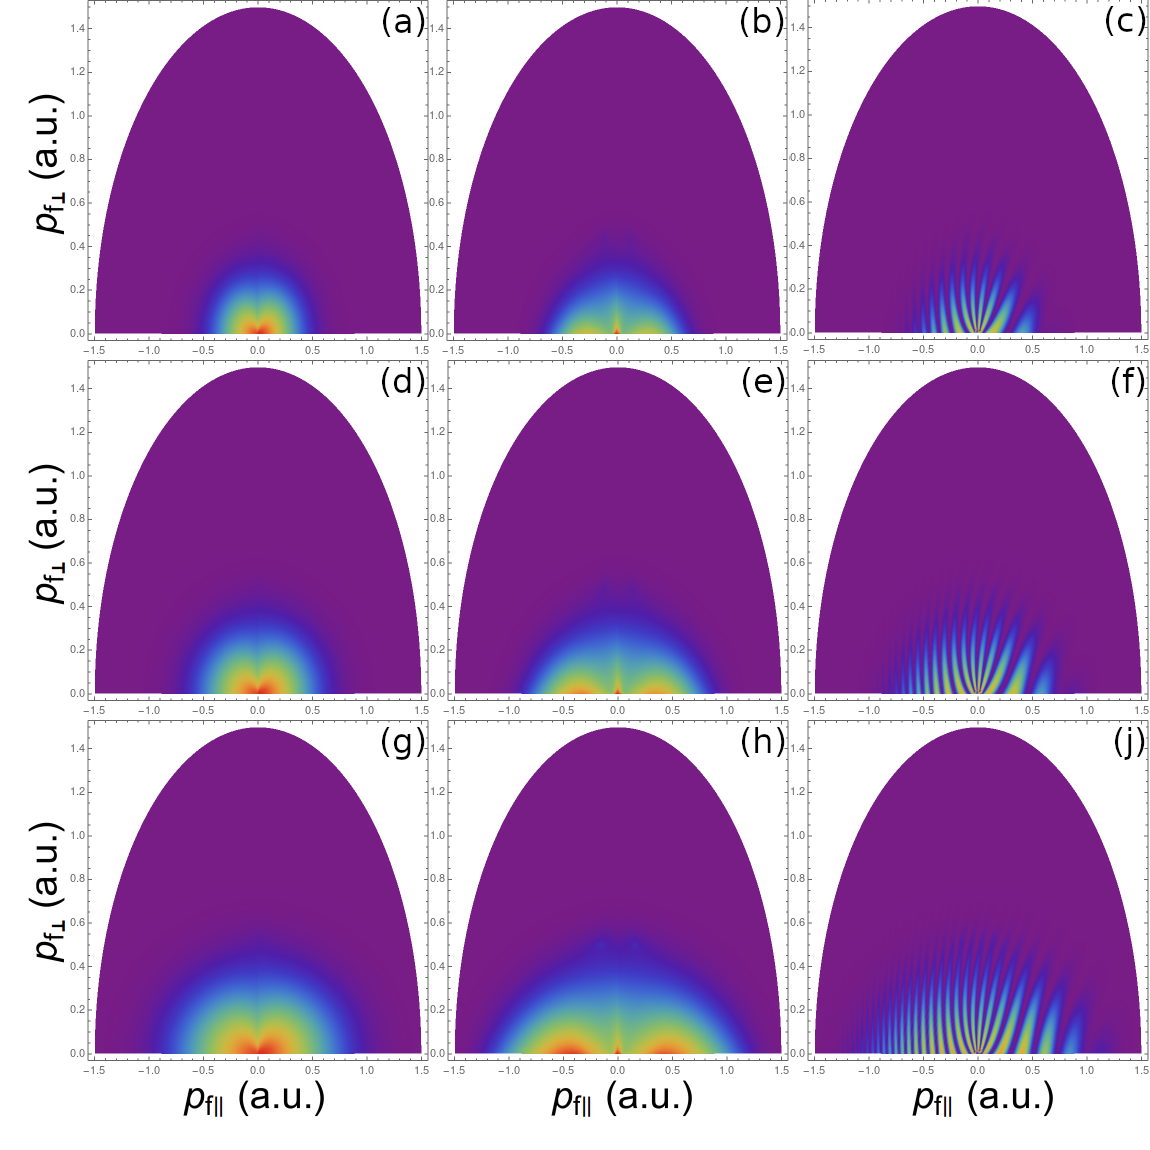
\includegraphics[width=14cm, height=10cm]{Figures/CQSFA_Interf.png}
    \caption{CQSFA momentum distributions for varying orbits and field intensities in a single field cycle. Panels (a)-(c) correspond to a field intensity of $I=5\cdot 10^{13} Wcm^{-2}$, panels (d)-(f) correspond to $I=1\cdot 10^{14} Wcm^{-2}$, while panels (g)-(f) correspond to $I=2\cdot 10^{14} Wcm^{-2}$.
    The first column, panels (a),(d),(g) show orbit 1, the middle column, panels (b),(e),(h) show orbit 2, and the right column, panels (c),(f),(j) show the interference of the complex transition amplitudes of orbits 1 and 2.}
    \label{fig:CQSFA_interf}
\end{figure}
\newline
Fig. \ref{fig:CQSFA_interf} shows the interference patterns obtained by considering orbit 1 and orbit 2 trajectories over a single cycle of the driving laser field. This interference is similar to the SFA, as $Im[t_1]$ and $Im[t_2]$ are comparable, and $Re[t_1]$ and $Re[t_2]$ follow the SFA solutions closely. Here the subscripts $1$ and $2$ refer to the orbit types. One can observe near vertical fringes, which get wider as one moves from negative to positive parallel momentum. The SFA background and analytic computations of the interference patterns was performed in (Maxwell et al., 2017)\cite{maxwell_2017_analytic}.
In the left and centre column showing orbits 1 and 2 respectively, the side lobes shown in Fig. \ref{fig:CQSFA_orb1_2} get wider as the field intensity increases from the top row towards the bottom.  Consequently, the interference patterns will widen as well, as seen form panels (c) to (f) to (j). The interference fringes reach farther in both parallel and perpendicular momentum regions, but for constant field wavelength they do not change their position or shape with varying field intensity.

\section{The Frankenstein Approximation}
The work presented in this section was done in close collaboration with my research partner and fellow MSci Theoretical Physics student, Tobin Holtmann. The derivation of the functional form of the Frankenstein model transition amplitudes, and the corresponding saddle point equations in Section \ref{ch:FEA} are mainly his work. The interpolation, computational solving method and numerical results presented in latter sections are my own work, except where acknowledged and referenced otherwise.
\par
The name 'Frankenstein Approximation' came about, as we seek to combine two paths of research in the same area. Although theoretically the two branches of research in ATI, NSDI and the CQSFA are theoretically similar, the frameworks developed for solving the problems are different, hence we found the nickname appropriate for the course of our MSci projects.

\subsection{Frankenstein Transition Amplitudes} \label{ch:FEA}

As discussed in Section \ref{ch:TSM}, the RESI is modelled as a three-step process, made up of tunnel ionisation and laser induced rescattering of the first electron, then the subsequent tunnel ionisation of the second electron. This process is represented in the Feynman diagram shown in Fig. \ref{fig:NSDI_feyn}. 
\begin{figure}[!htb]
    \centering
    \includegraphics[width = 14cm,height=6cm]{Figures/diagram-20200406.png}
    \caption{Feynman diagram corresponding to the RESI process.}
    \label{fig:NSDI_feyn}
\end{figure}
\newline
This Feynman diagram, together with the appropriate substitutions made based on the Strong Field Approximation, leads to the final transition amplitude as a function of the two-electron final momentum states
\begin{equation} \label{}
   M_{RESI}(\mathbf{p_1},\mathbf{p_2}) = \int_{-\infty}^{\infty}dt_3\int_{-\infty}^{t_3}dt_2\int_{-\infty}^{t_2}dt_1\\ d^3\mathbf{k} V_{\mathbf{p}_2e}V_{\mathbf{p}_1e,\mathbf{k}g}V_{\mathbf{k}g}
   e^{iS(\mathbf{p_1},\mathbf{p_2},\mathbf{k},t_1,t_2,t_3)}
\end{equation}
with the action given by 
\begin{multline} \label{eq:NSDIaction}
    S^{RESI}(\mathbf{p_1},\mathbf{p_2},\mathbf{k},t_3,t_2,t_1) = -\int_{t_3}^{\infty} d\tau \frac{[\mathbf{p}_2 + \mathbf{A}(\tau)]^2}{2} - \int_{t_2}^{\infty} d\tau \frac{[\mathbf{p}_1 + \mathbf{A}(\tau)]^2}{2} \\
    - \int_{t_1}^{t_2} d\tau \frac{[\mathbf{k} + \mathbf{A}(\tau)]^2}{2} + E_{2e}(t_3-t_2) + E_{2g}t_2 + E_{1g}t_1
\end{multline}

The basis of the Frankenstein approximation is that this action is separable into terms corresponding only to the first electron, and terms corresponding only to the second electron. The prefactors for the NSDI are defined in equations Eq. (\ref{eq4}) - Eq. (\ref{eq6}). In particular,  $V_{\mathbf{p}_1e,\mathbf{k}g}$ given by Eq. (\ref{eq6}) depends on both electrons. Because the problem is solved using the Saddle Point Approximation, the assumption was made both in the NSDI and in the CQSFA calculations that the prefactors vary much slower than the complex exponential $e^{iS(\mathbf{p_1},\mathbf{p_2},\mathbf{k},t,t',t'')}$. This means that the prefactors may lead to enhancement or suppression in certain ranges of final momentum distribution, but the general shape of the distribution will be determined by the action given in Eq. \ref{eq:NSDIaction}. For this reason we consider only the action for the calculation of the transition amplitudes, with the prefactors assumed to be unity. This simplification can only be done under specific circumstances, and usually for more complex calculations and interference patterns the prefactors also need to be considered. Most importantly, this only works if a single ionisation channel is considered, because the relative amplitudes of the different channels are contained in the prefactors.
\par
We then continue by identifying terms in the action corresponding to the second electron, and seek to replace them with the action corresponding to the CQSFA Eq. (\ref{eq:terms_action}) to obtain the final two-electron transition amplitudes as a function of their final momenta. The Feynman diagram corresponding to this process is illustrated in Fig. \ref{fig:FRANK_feyn}
In the same notation as RESI, the CQSFA action Eq. (\ref{eq:NSDIaction}) for the second electron reads as
\begin{multline} \label{eq:CQSFAaction}
    S^{CQSFA} (\tilde{\mathbf{p}}, \mathbf{r}, t_{3r}, t_3, t_f) = E_{2e}(it_{3i}) -  \int_{t_3}^{t_{3r}} d\tau \frac{[\mathbf{p_0} + \mathbf{A}(\tau)]^2}{2} - \int_{t_3}^{t_{3r}} d\tau V(\mathbf{r_0}(\tau))  \\
    + E_{2e}(t_{3r}) -\int_{t_{3r}}^{t_f} d\tau \frac{[\mathbf{p}(\tau) + \mathbf{A}(\tau)]^2}{2} - 2 \int_{t_{3r}}^{t_f} d\tau V(\mathbf{r}(\tau)) 
\end{multline}
where the first 3 terms correspond to the tunnel ionisation, and the last 3 terms to the propagation to the detector after ionisation. As discussed in Section \ref{ch:CQSFA}, this separation of terms is most useful to illustrate the calculation contour taken in the complex plane $t_3 \rightarrow t_{3_r} \rightarrow t_f$, analytically the expression can be combined into just 3 terms with the integrals going from $t_3$ to $t_f$.
\begin{figure}[!htb]
    \centering
    \includegraphics[width = 14cm, height=6cm]{Figures/Frankenstein_feynman.png}
    \caption{Modified Frankenstein Feynman diagram, including the effect of the Coulomb potential on the second electron.}
    \label{fig:FRANK_feyn}
\end{figure}
\newline
The RESI action in Eq. (\ref{eq:NSDIaction}) can be split into two terms
\begin{equation}
    S^{RESI}(\mathbf{p_1}, \mathbf{p_2}, \mathbf{k}, t_1, t_2, t_3, t_f) = S_A(\mathbf{p_1},\mathbf{k}, t_1, t_2) + S_B(\mathbf{p_2},t_3, t_f)
\end{equation}
with 
\begin{equation}
    S_A(\mathbf{p_1},\mathbf{k}, t_1, t_2) = - \int_{t_2}^{\infty} d\tau \frac{[\mathbf{p}_1 + \mathbf{A}(\tau)]^2}{2} \\
    - \int_{t_1}^{t_2} d\tau \frac{[\mathbf{k} + \mathbf{A}(\tau)]^2}{2} + E_{1g}t_1 + (E_{2g} - E_{2e})t_2
\end{equation}
and
\begin{equation} \label{eq:SB}
    S_B(\mathbf{p_2},t_3, t_f) = -\int_{t_3}^{t_f} d\tau \frac{[\mathbf{p}_2+\mathbf{A}(\tau)]^2}{2} + E_{2e}t_3
\end{equation}
where $S_A(\mathbf{p_1},\mathbf{k}, t_1, t_2)$ and $S_B(\mathbf{p_2},t_3, t_f)$ only depend on the first and the second electron, respectively. In Eq. (\ref{eq:SB}) the integration limit was changed from $\infty$ to $t_f$. This makes no change in the context of NSDI, as the field dressed momentum in the Volkov states is conserved. In the CQSFA, the momentum is not conserved due to the influence of the Coulomb potential. In the analytical expressions the limit $t_f \rightarrow \infty$ is considered. in practice this is achieved by choosing $t_f$ to be several (in most calculations around 20) field cycles later than $t_3$. At such times, the electrons have enough time to propagate sufficiently far away from the core that the effect of the Coulomb potential becomes negligible. We can then replace $S_B$ with Eq. (\ref{eq:CQSFAaction}) to give the final Frankenstein action as
\begin{equation} \label{eq:FRANKAction}
    S^{FR}(\mathbf{p_1}, \mathbf{p_2}, \mathbf{k}, t_1, t_2, t_3, t_f) = S_A(\mathbf{p_1},\mathbf{k}, t_1, t_2) + S^{CQSFA} (\mathbf{p_2}, \mathbf{r}, t_{3r}, t_3, t_f)
\end{equation}
We seek to find the solutions to $t_1, t_2, t_3$ and $\mathbf{k}$ using the saddle point method, as before. Since the functional form of the action is unchanged from the NSDI and the CQSFA parts, the derivatives with respect to each of the variables, and hence the saddle point equations will have the same form. The saddle point equations become
\begin{equation}\label{eq:sad1}
    \frac{\partial S}{\partial t_1} = 0 \Rightarrow [\mathbf{k} + \mathbf{A}(t_1)]^2 = -2E_{1g}
\end{equation}
\begin{equation}
    \frac{\partial S}{\partial t_2} = 0 \Rightarrow -[\mathbf{k} + \mathbf{A}(t_2)]^2 + [\mathbf{p_1} + \mathbf{A}(t_2)]^2 = -2(E_{2e} - E_{2g})
\end{equation}
\begin{equation}
    \frac{\partial S}{\partial \mathbf{k}} = 0 \Rightarrow - \frac{1}{t_2 - t_1} \int_{t_1}^{t_2} \mathbf{A}(\tau) d\tau
\end{equation}
\begin{equation}\label{eq:sad4}
    \frac{\partial S}{\partial t_3} = 0 \Rightarrow [\mathbf{p_0} + \mathbf{A}(t_3)]^2 + 2 V(\mathbf{r}(t_3)) = -2E_{2e}
\end{equation}
\newline
In terms of the solutions to the saddle point equations, the Frankenstein transition amplitude can be written as
\begin{multline}
    M_{FR}(\boldsymbol{p}_{1} ,\boldsymbol{p}_{2}) =i{\displaystyle ( 2\pi )^{3}\lim _{t_{f}\rightarrow \infty }\sum _{s}\left\{\det\left[\frac{\partial \boldsymbol{p}_{s}( t_f)}{\partial \boldsymbol{r}_{s}( t_{3s})}\right]\right\}^{-1/2}} \\
    \times \frac{{\displaystyle } V_{\mathbf{p_0}e}( t_{3s} ,\boldsymbol{p}_{0}) V_{\mathbf{p_1}e,\mathbf{k}g}( t_{2s} ,\boldsymbol{p_1} ,\boldsymbol{k}( t_{1s} ,t_{2s})) V_{\mathbf{k}g}( t_{1s} ,\boldsymbol{k}( t_{1s} ,t_{2s}))}{\sqrt{( t_{3s} -t_{2s})^{3}\det[ S''(\boldsymbol{p}_{1} ,\boldsymbol{p_{s} ,r_{s} ,k} ,t_{1s} ,t_{2s} ,t_{3s} ,t_{f})]}} \\
    \times exp[iS(\boldsymbol{p}_{1} ,\boldsymbol{p_{2} ,k}( t_{1s} ,t_{2s}) ,t_{1s} ,t_{2s} ,t_{3s} ,t_{f})]
\end{multline}
with the prefactors given by the suitable forms of Eq. (\ref{eq4}), Eq. (\ref{eq6}) and Eq. (\ref{eq:prefactor}).

\subsection{Coherent and Incoherent Sums}
The final result we aim to work towards is a map of transition probabilities for each point in 2D momentum space, where the axes represent the momenta of electron 1 and electron 2 parallel to the laser field polarisation. This involves integrating over the perpendicular momenta of the electrons i.e.
\begin{equation}\label{eq:W}
    W(p_{1\parallel}, p_{2\parallel}) = \int \int d^2p_{1\perp} d^2p_{2\perp}\left | M_{FR}(\mathbf{p_1}, \mathbf{p_2}) \right |^2
\end{equation}
where
\begin{equation} \label{eq:MFR}
    \left |M_{FR}(\mathbf{p_1}, \mathbf{p_2})\right |^2 =\left | M_{RESI}(\mathbf{p_1}) \cdot M_{CQSFA}(\mathbf{p_2}) \right |^2
\end{equation}
This equation can be separated only if we are considering a single ionisation channel, and a single quantum orbit for electron 2. If we are considering multiple channels, Eq. \ref{eq:W} becomes 
\begin{equation}\label{eq:Wcoh}
    W^{(COH)}(p_{1\parallel}, p_{2\parallel}) = \int \int d^2p_{1\perp} d^2p_{2\perp}\left | \sum_c M^{(c)}(\mathbf{p_1}, \mathbf{p_2}) \right |^2
\end{equation}
where the superscript $c$ refers to the different ionisation channels considered.
The transition probability $ W(p_{1\parallel}, p_{2\parallel})$ can be in this case can be computed by summing coherently or incoherently over the complex amplitudes of the different channels. The coherent sum is given in Eq. \ref{eq:Wcoh}, where the complex amplitudes are added together, and the square magnitude of the result is taken afterwards to give the transition probability. In the incoherent calculation the square modulus of the complex amplitude is taken before summing over the channels, which leads to
\begin{equation}
    W^{(INCOH)}(p_{1\parallel}, p_{2\parallel}) = \int \int d^2p_{1\perp} d^2p_{2\perp} \sum_c \left | M^{(c)}(\mathbf{p_1}, \mathbf{p_2}) \right |^2
\end{equation}
Furthermore, interference between multiple types of orbits of the second electron can be considered, or same types of orbits but released in different field cycles. In this case the expression for the transition amplitude squared becomes 
\begin{equation} \label{eq:Mfr}
    \left |M_{FR}(\mathbf{p_1}, \mathbf{p_2})\right |^2 =\left | M_{RESI}(\mathbf{p_1}) \right | ^2 \cdot \left | \sum_i M_{CQSFA}^{(i)}(\mathbf{p_2}) \right |^2
\end{equation}
where the superscript $i$ refers to the orbit of the second electron. This summation again can be computed coherently and incoherently. 
\subsection{Interpolation Method}
Another challenge faced is the discretisation of the momentum space we are working with. The framework for solving the Saddle Point Equations and calculate the transition amplitudes for individual momentum points is set in polar coordinates. It was originally a feature of the CQSFA framework and solver developed by Andrew Maxwell, as polar coordinates make distinguishing orbits simpler. It also avoids calculating regions too far away from the origin in the corners of a Cartesian momentum grid. This poses a problem, as the perpendicular momentum components that we wish to integrate over are defined in Cartesian coordinates. On a Cartesian grid, such integration can be performed by a discrete summation. In the polar grid, the discrete points of known values do not line up with the discrete parallel momentum points that we want to keep as the only final variable. Furthermore, in the polar grid there is oversampling in the middle of the distribution close to the origin, where the radial "spokes" of solved points, lie much closer together, which would make integration even more troublesome.
\par
Our solution to this problem was to solve the saddle point equations and compute the action on high resolution momentum grids in polar coordinates. Then we superimpose a Cartesian grid and calculate each of the points using interpolation. We chose the simple method of linear interpolation because the first order interpolation was likely to be sufficiently accurate, as long as the resolution of both the input polar and the output Cartesian grids is high enough. The interpolation method tessellates the input point set to n-dimensional simplices, then interpolates linearly on those simplices. Then on the Cartesian grid the integration can be replaced with a discrete sum over all the perpendicular momentum points corresponding to a value of parallel momentum.
\par
Interpolation also performs the task of matching the discretisation of the separate solutions, by imposing the same Cartesian grid on the individually computed solutions of electron 1 and electron 2. This step is crucial in order to be able to calculate coherent sums between different solutions.

\subsection{Computational Method} \label{ch:comp_method}
For both the NSDI and the CQSFA, there already existed numerical solving programs written in C++, that were provided to us by our supervisor Dr. C. Faria, Andrew Maxwell, and other past and present members of their research group in ATI. My work was to identify the relevant parts of the projects that were useful for the Frankenstein calculations, and perform necessary modifications, and to combine parts to yield the sought results. I had to modify the momentum parameters used throughout the NSDI solver, to adapt it to a polar grid to match the CQSFA. I wrote the code in Python that performs the regularisation of the momentum grids, performs the necessary interpolations, integrates over the perpendicular momentum components and combines the results. The results were plotted using Wolfram Mathematica.
\par
The calculation of the action and transition amplitudes was performed in parts by the respective solving programs, as we had to build the final Frankenstein action by merging the SFA and CQSFA approaches for electrons 1 and 2, respectively. Since the action is factorisable, the terms in the exponent corresponding to the two electrons could be calculated independently. As we have seen in Section \ref{ch:RESI}, in the NSDI there is no distinction between final an initial momenta of the second electron, as the field-dressed momentum in the Volkov states is conserved. However, in the CQSFA it is not the case, which leads to us having to solve the inverse problem for the second electron where the initial momentum is calculated from the final momentum. When considering a multiple events, causality also needs to be taken into account. As in the RESI, the time ordering operator $\mathcal{T}$ is used to make sure the second electron ionises after the first electron returns. When considering a single event in linearly polarised monochromatic light, one can always allow the first electron to rescatter, and pick a subsequent field maximum for the second electron to ionise, as the field is periodic $\mathbf{E}(t) = \mathbf{E}(t+\frac{2\pi}{\omega})$.
\par
Then, using the properties of exponentials, the transition amplitude for each of the two-electron final momentum pairs could be calculated, for a single event, as the product of the corresponding final momentum points for each of the electrons separately.
\begin{figure}[!htb]
    \centering
    \includegraphics[width=14cm]{Figures/e1_2_line.png}
    \caption{Separable momentum distributions for factorisable action. Panel (a) and panel (b) show transition probabilities for electron 1 and electron 2 as a function of their parallel momentum component, respectively. Panel (c) shows the combined momentum map of the 2-electron process, including symmetrisation.}
    \label{fig:lines}
\end{figure}
\newline
This is shown in Fig. \ref{fig:lines}. Panels (a) and (b) show the transition probability of electrons 1 and 2 individually. In these plots the interpolation onto a Cartesian grid and integration over perpendicular momentum components were already carried out, so the only independent variable remains the parallel momentum component of each electron. These transition probabilities are then combined by taking the outer product of the two vectors containing the transition probabilities related to each electron, which is shown in panel (c). In this panel the symmetry operation $(\mathbf{p_1},\mathbf{p_2}) \leftrightarrow (\mathbf{p_2},\mathbf{p_1})$ was performed, as the two electrons are indistinguishable at the detector.

\subsection{Single Channel Single Orbit}

The simplest model we investigated is a single ionisation channel and a single CQSFA orbit for the second electron. Without considering prefactors and for a single channel, the transition amplitude given by Eq. \ref{eq:MFR} is separable to terms related only to the first and only to the second electron. The partial transition amplitudes for each electron were calculated separately, by solving the saddle point equations Eq. \ref{eq:sad1} - Eq. \ref{eq:sad4}, and inserting the solutions into the respective terms of the Frankenstein action Eq. \ref{eq:FRANKAction}. Then interpolation was used to transform the distributions to a Cartesian grid in momentum space, where the perpendicular momentum components of each electron, $p_{1\perp}$ and $p_{2\perp}$ were integrated over as shown in Eq. \ref{eq:W}. The results are shown in Fig. \ref{fig:single_orbit_5e13}.
\begin{figure} [!htb]
    \centering
    \includegraphics[width = 14cm]{Figures/combined_800_5e13.png}
    \caption{Final electron momentum distributions calculated for Argon, with a linearly polarised laser field of wavelength $\lambda = 800nm$, and intensity $I = 5*10^{13} Wcm^{-2}$.The markings on the axes are in the units of $U_p$. In panel (a) the SFA calculation was used for the RESI process. Panel (b) and (c) show the Frankenstein calculation with CQSFA orbit 1 and orbit 2, respectively. The magnitude of each plot has been normalised relative to the highest value.}
    \label{fig:single_orbit_5e13}
\end{figure}
\newline
In panel (a), the distributions show two key features of the SFA three-step model. As discussed in Section \ref{ch:RESI_mom}, the first electron is likely to ionise with vanishing parallel momentum, and after rescattering it reaches the detector with nonvanishing momentum parallel to the laser field polarisation. Secondly, the second electron also undergoes a tunnel ionisation process, hence it is also most likely to ionise with vanishing parallel momentum. Since the two electrons are indistinguishable at the detector, a momentum swap $M(\mathbf{p_1}, \mathbf{p_2}) \leftrightarrow M(\mathbf{p_2}, \mathbf{p_1})$. 
In panels (b) and (c) the general shape of the SFA distribution is obtained, regions of transition along the axes, centred at nonvanishing momenta. However, for orbit 1 in panel (b), the suppression in the centre can be observed. As discussed in Section \ref{ch:Single_CQSFA}, in the CQSFA the second electron is no longer likely to tunnel ionise with vanishing parallel momentum component, as it needs to overcome the binding potential to reach the detector. The narrowing of the distributions is also due to the second electron, the parallel momentum region where the first orbit manifests is localised closer to zero. For orbit 2 in panel (c), similar side lobes can be observed, but they are wider than those of orbit 1. A region of high transition probability is visible along the axes, which is a consequence of the way the action is calculated, and it would be suppressed by the prefactors\cite{maxwell_2017_coulombcorrected}. These features correspond to the second electron tunnel ionisation predicted using the CQSFA, shown in Fig. \ref{fig:CQSFA_orb1_2}.
\par
These results correspond to the simplest case of a single field cycle and a single orbit considered, but they illustrate the main changes compared to the SFA, the narrowing and splitting of the momentum regions where transition is likely.

\subsection{Two-Orbit Interference}\label{ch:two_orbit}

As discussed in Section \ref{ch:CQSFA_interf}, interference between different quantum trajectories of the second electron can be observed. Mathematically, these interference patterns can be obtained by considering Eq. (\ref{eq:Mfr}), where the complex amplitudes of electron 1 and electron 2 are summed incoherently, but the different solutions of the saddle point equations that lead to orbits 1 and 2 of the second electron are considered coherently. This is a valid solving method, as we are considering a single event, therefore there is no inter-cycle interference between electron 1 and electron 2..
\begin{figure}[!htb]
    \centering
    \includegraphics[width=14cm]{Figures/Frank_800_5e13_3up_orb12_interf.png}
    \caption{Interference in the Frankenstein approximation for monochromatic field with wavelength $\lambda = 800nm$ and intensity $I=5\cdot10^{13}Wcm^{-2}$. Panels (a) and (b) show the parallel momentum distributions in the Frankenstein model for the second electron orbit 1 and orbit 2, respectively. In panel (c) the interference of the two is shown.}
    \label{fig:frank_inter}
\end{figure}
\newline
In Fig. \ref{fig:frank_inter} this interference was illustrated for an intensity of $I=5\cdot10^{13}Wcm^{-2}$. Interference fringes can be seen running parallel to the axes, which arises form the interfering orbits of the second electron. More precisely, it is the effect of integrating over the perpendicular momentum component of Fig. \ref{fig:CQSFA_interf} panel (c). There the fringes at negative parallel momenta run along the perpendicular momentum axis, while they are tilted at positive parallel momenta. Consequently, after the integration over the perpendicular momenta in Fig. \ref{fig:frank_inter} shows sharper fringes towards the negative parallel momentum side of the distributions, and more washed-together fringes towards positive parallel momenta. 

\subsection{Further Work}

As shown in Fig. \ref{fig:frank_inter}, even without considering prefactors and only considering a single field cycle, we can obtain traces of the quantum interference patterns found in ATI, using the Coulomb Quantum-orbit Strong Field Approximation. In order to be able to calculate more transition probabilities for more complex setups, such as multiple cycles or multiple ionisation channels, some further modifications to our method will be needed. 
\par
The most significant drawback of our approach is the need to use interpolation to switch between polar and Cartesian coordinate bases. Although for high resolution computations it yields reasonably accurate results, it may introduce unwanted artefacts. It does not allow us to consider fully coherent summation of the complex transition amplitudes of the first and second electron, and hence consider interference between different events in multiple field cycles. Although for a single cycle, it is possible to consider interference of multiple orbits of the second electron in polar coordinates and then interpolate the square amplitude, for coherent summation this does not work. Because the solved values need to be on the same grid, coherent summation would require us to interpolate both the imaginary and the real components of the transition amplitudes of both electrons separately, before being able to sum them together in the same Cartesian coordinate basis. This causes problems, because the imaginary and real components $\mathcal{I}m[M(\mathbf{p_i})]$ and $\mathcal{R}e[M(\mathbf{p_i})]$ of the amplitudes vary much quicker than the probability $\left | M(\mathbf{p_i}) \right |^2$. Having to perform 4 interpolations, on much more quickly quantities, leads to a significant decrease in the accuracy of the results, where it is no longer possible to distinguish between interference features and computational artefacts. Interpolation also performs poorly at the more quickly varying patterns at higher intensities, which prevented us from exploring a wider intensity range computationally.
\newline
The most ideal solution to this problem would be to cast both of the problems in Cartesian coordinates, hence removing the need for interpolation, and allowing one to perform coherent and incoherent summations freely. The SFA solving program for the first electron is already available in Cartesian coordinates. In the beginning of the project we decided to adapt that to the polar coordinate system of the CQSFA code, as the latter is computationally much more complex and is mathematically more complicated to change. For future work, one would need to do the opposite, and solve the CQSFA equations in Cartesian coordinates.
\par
If one wishes to consider events over multiple field cycles, the time ordering of the events will also need to be considered. As mentioned in Section \ref{ch:comp_method}, causality dictates that the second electron tunnels after the first electron rescatters, and hence promotes it to an excited state. For multiple cycles, one needs to carefully consider which rescattering event leads to the excitation of which electron, and determine which electrons may or may not interfere.
\par
Finally, although the prefactors do not change the dynamics of the interference patterns, they still have a strong influence by enhancement or suppression in various momentum regions. Furthermore, they are necessary if one wants to consider interference between multiple ionisation channels, as they contain the relative intensities of patterns that correspond to the different values of energy levels and ionisation potentials. These prefactors may be formulated in terms of the ionisation time solutions of the saddle point equations, $t_1$, $t_2$, $t_3$ and the intermediate momentum state $\mathbf{k}$. Some of the prefactors, however, are not factorisable to terms corresponding to the individual electrons. For this reason, to consider the prefactors, one needs to solve the saddle point equations in a single combined framework, which then allows for the calculation of their values.

\section{Summary}

After a brief introduction and history of ATI, we considered some important mathematical devices used in calculations throughout the project. We discussed experiments that lead to discovery of Nonsequential Double Ionisation (NSDI), and to the the inception of the three-step model. It was shown that this model can lead to multiple ATI processes, including Rescattering Excitation with Subsequent Ionisation (RESI), which is a nonsequential process involving two active electrons. We discussed how the process is currently treated through the use of the Strong Field Approximation (SFA), and introduced some results from computational solving methods. Then we were exploring the main shortcoming of the SFA, as it disregards the effect of the Coulomb potential in most of the calculations. We showed how the equations governing the RESI process can be factorised in terms dependent on each of the electrons separately. 
\par
Then we introduced the Coulomb Quantum-orbit Strong Field Approximation (CQSFA), which is a model that seeks to improve upon the Strong Field Approximation, by considering the effect of the Coulomb potential on the continuum sate electrons. We introduced the mathematical background of the model, the ways it improves upon the SFA, and how solutions can be calculated in practice. We presented some results for simple setups, and showed how interference patterns arise in this model.
\par
Finally, we showed how the RESI equations can be modified to include the improvements of the CQSFA model. We found that in simple cases, one can simplify the equations by only considering the action, without the prefactors to obtain final momentum distributions of the two electrons. We explored in what circumstances it can be used, and presented some results for individual orbits, and even simple interference between different quantum trajectories of the second electron. We also identified the necessary modifications to our approach that can be made to improve the model, and to extend the applicability to processes involving multiple laser field cycles and multiple ionisation channels.

\section{Acknowledgements}
First and above all else, I would like to express my gratitude to my supervisor Dr. Carla Faria, for supporting me throughout the project. Next, I would like to acknowledge the works of Andrew Maxwell, and Abbie Bray for helpful discussions and help. I would also like to acknowledge the works of Ahmed Al-Jawahiry and Tahir Shaaran, whose works provided the groundwork and inspiration for the project. Finally, I would like to thank my research partner and good friend Tobin Holtmann, together with whom we tackled many challenges of the project.
\newpage
\printbibliography
\end{document}